% !TEX root = main.tex
\chapter{Decay-time fit}
\label{chap:dectimeFit}

\linespread{1.08}\selectfont
In this chapter the decay-time fit on \BdToDpi to extract the \CP observables \Sf and \Sfbar is presented.
Section \ref{sec:resolution} and \ref{sec:acceptance} describe the parameterisation of the decay time resolution and acceptance before the extraction of the \CP parameters is presented in \cref{sec:ExtractCPobs}.
The validation of the fit is detailed in \cref{sec:decTimeFitVal}.
After comparing the resulting values of nuisance parameters with reference values, the \emph{link function} used for the calibration function of the OS and SS taggers is validated (\cref{sec:ValLinkFunction}).
At last, the fit to extract the \CP parameters is repeated on different sub samples of the data set (\cref{sec:valOnSub Sample}) and the entire strategy is also tested on simulated events (\cref{sec:valOnSim}).

\section{Fit to data}

In the following, the decay-time fit to extract \Sf and \Sfbar and its components are presented.
The fit is performed on the decay-time range from \SIrange{0.4}{12}{\pico\second}.
The lower limit was chosen in order to obtain a good description of the decay-time distribution at low decay-times without losing sensitivity to the parameters \Sf and \Sfbar.
The upper limit was set to a value such that the statistics is already too small so that an enlarged range would no longer add sensitivity to the \CP parameters.

\subsection{Decay time resolution}
\label{sec:resolution}

Since the work in this section was done by a collaborator, the contents are described only briefly.

The decay-time resolution is determined on a sample of \emph{fake} \Bz candidates, formed from a prompt \Dpm candidate and another track originating from the PV.
These \emph{fake} \Bz candidates are expected to have a decay time of zero and therefore the sample also is referred to as prompt sample.
The candidates are selected with the same selection as presented in \cref{sec:selection}, except for the cut on the BDT output.
Additionally, the \emph{fake} \Bz candidates are required to have an \chisqip with the PV less than nine and the number of \ac{PV}s in the event must be one to exclude wrong \ac{PV} associations.
Subsequently, \emph{sWeights}~\cite{Pivk:2004ty} are determined by a fit to the invariant mass of the \Dpm meson in order to examine only signal distributions in the following.
Since the time resolution depends on the transverse momentum of the bachelor particle, this needs to be corrected in the sample of \emph{fake} \Bz candidates.
Therefore, the prompt sample is weighted by the ratio of the distributions of the logarithmic transverse momenta of the bachelor candidate in the signal \BdToDpi and the prompt sample.

To resolve the decay-time resolution, fits are then performed to the decay-time distribution of the prompt sample in \num{20} bins of the decay-time error.
Since this sample does not contain real \Bz candidates, the decay-time resolution can be derived from the width of the decay-time distribution.
The binning is chosen such that the sum of \emph{sWeights} in each bin is equal.
The fit model consists of three components: a delta function convolved with a Gaussian function to describe true prompt \Dpm+track candidates, a pair of exponential functions convolved with the same Gaussian function to describe candidates from \bquark hadrons and a wide Gaussian function to describe backgrounds due to wrongly associated \ac{PV}s.
The fit is shown for one representative bin in \cref{fig:resolutionRepresentativeBin}.
\begin{figure}[tbp]
    \centering
    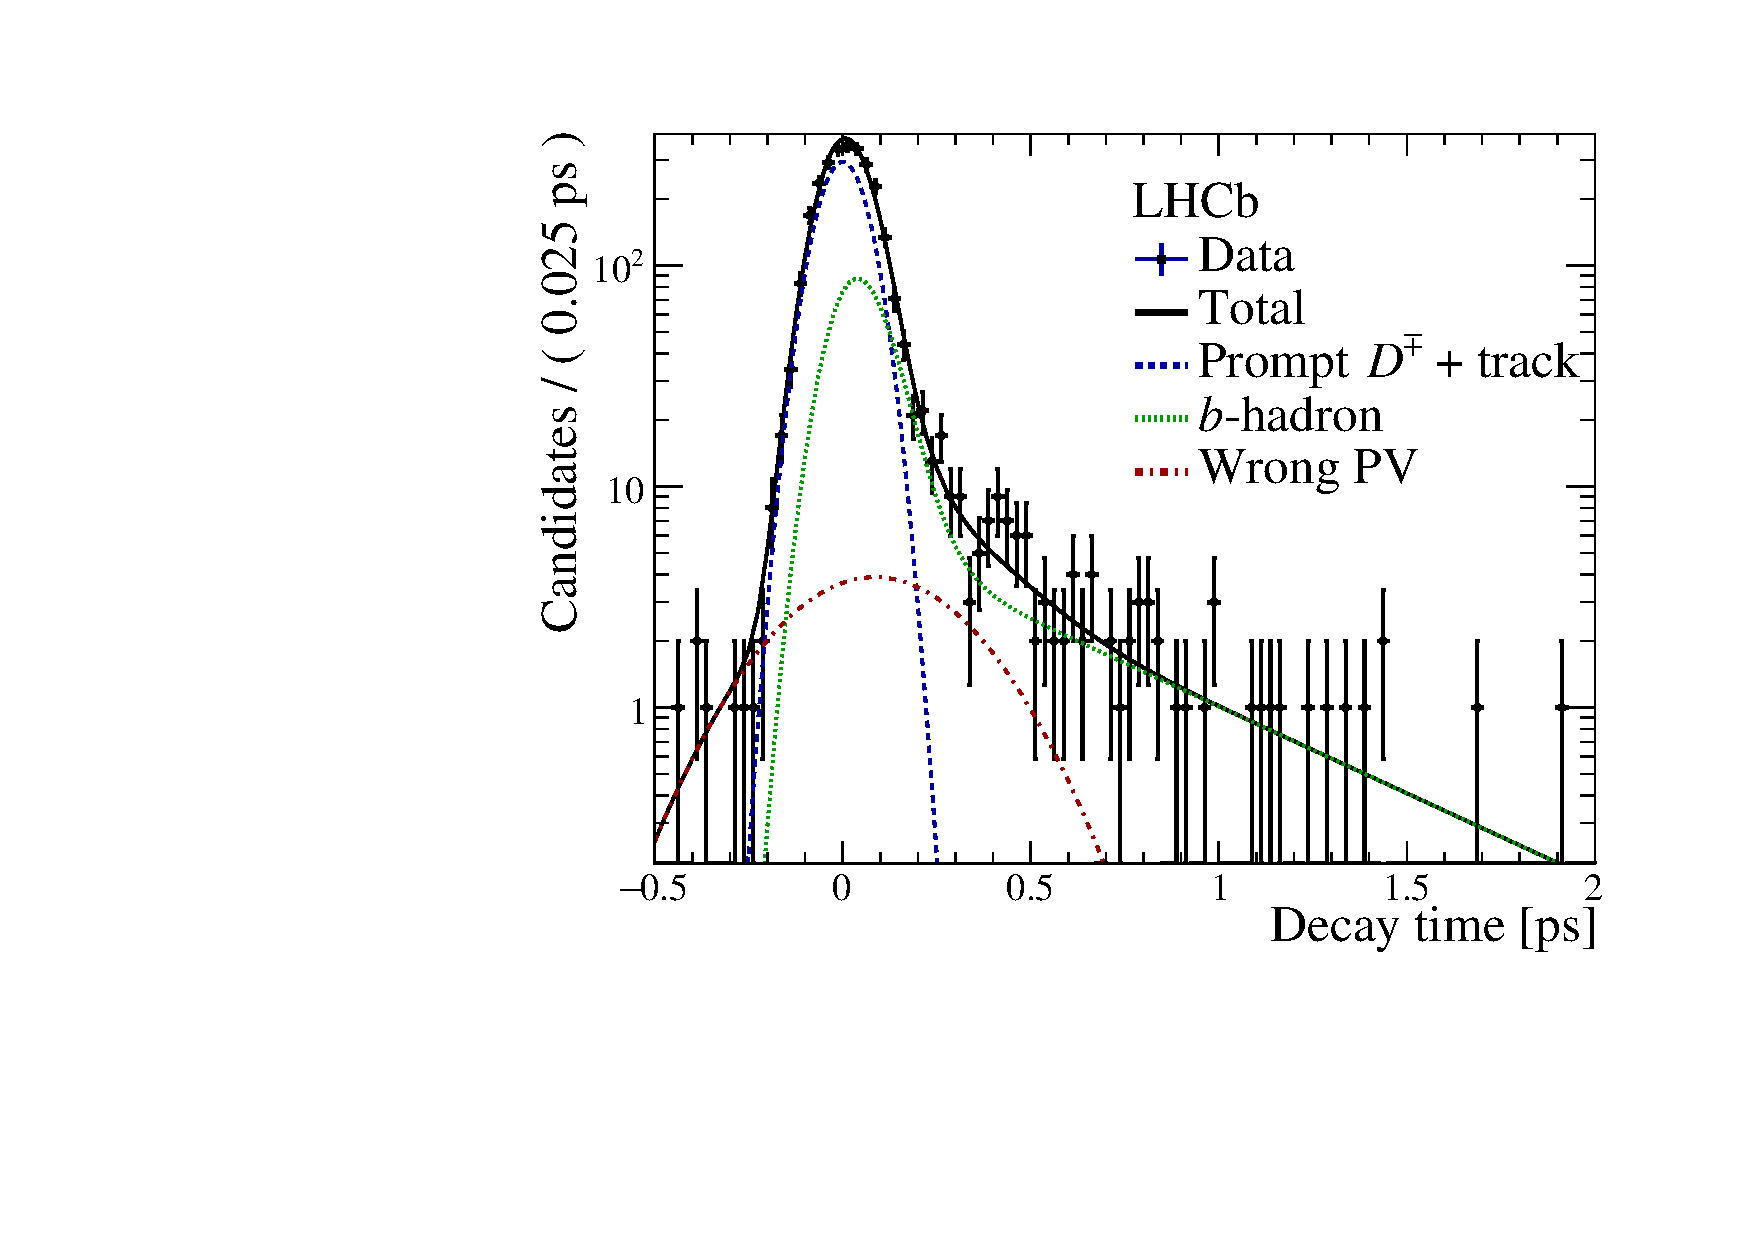
\includegraphics[width=0.48\textwidth]{10TimeFit/figs/resolution_Bin15.pdf}
    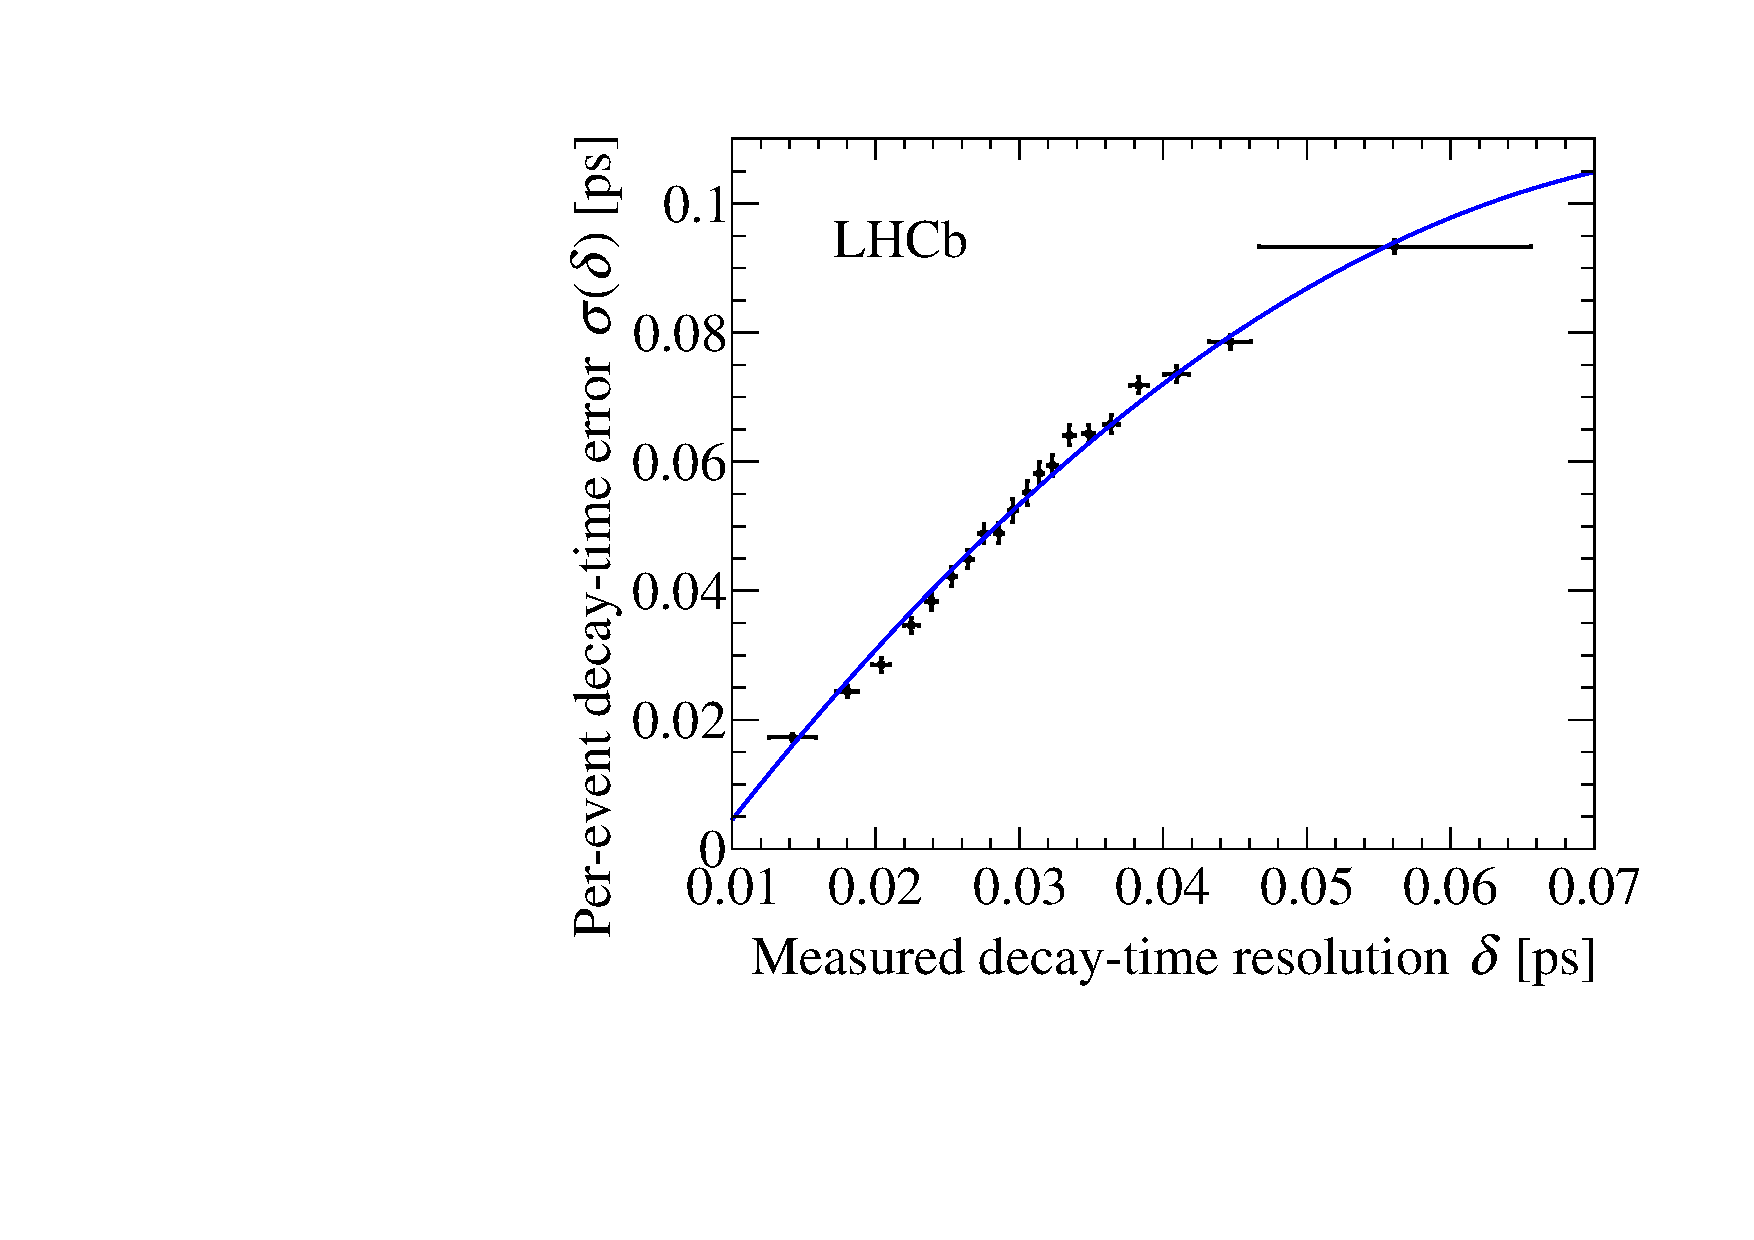
\includegraphics[width=0.48\textwidth]{10TimeFit/figs/resolution_chi2Fit.pdf}
    \caption{Distribution of the decay-time resolution for one representative bin in per-candidate decay-time error for \emph{fake} \Bz candidates (left) and measured resolution versus average per-candidate decay-time error, determined from fits to the decay time in bins of decay-time error (right).}
    \label{fig:resolutionRepresentativeBin}
\end{figure}
A measured resolution $\left<\sigma\right>_i$ per bin is obtained from this fit, which can be related to the corresponding average decay-time error $\left<\delta\right>_i$.
Following, a $\chi^2$ fit to the $(\left<\delta\right>_i, \left<\sigma\right>_i)$ pairs of the form
\begin{equation}
\left<\sigma\right>_i=\left<\sigma\right>+p_1\times\left(\left<\delta\right>_i-\left<\delta\right>\right)+p_2\times\left(\left<\delta\right>_i-\left<\delta\right>\right)^2
\end{equation}
is performed, where $\left<\delta\right>$ is the average per-event decay-time error of the whole unbinned sample.
This $\chi^2$ fit is shown in \cref{fig:resolutionRepresentativeBin}.
It provides an average decay time resolution $\left<\sigma\right>$ and a trend, from which a global average resolution of \mbox{$\sigma\!\left(\left<\delta\right>\right)=\SI{54.91\pm0.38}{\femto\second}$} is determined.

\subsection{Decay-time dependent efficiency}
\label{sec:acceptance}

Due to \eg some selection criteria and trigger requirements, as well as inefficiencies in the \velo reconstruction, the detector efficiency is not constant over the \Bz decay-time.
This efficiency, referred to as acceptance $a(t)$, decreases very quickly towards zero for low decay times, reaches a plateau for intermediate decay times, and slightly drops again at high decay times.

For this analysis, two models were developed in parallel, which give almost identical results for the \CP parameters \Sf and \Sfbar.
The model used in the final decay-time fit was developed by a collaborator and has an additional degree of freedom, while the model described below is used as a crosscheck and for estimating systematic uncertainties.
In both models, the acceptance is parametrised by splines, which are implemented analytically in the decay-time fit as described in Ref.~\cite{Karbach:2014qba}.
These splines consist of cubic polynomials defined piecewise in decay-time.

The final acceptance parameterisation is characterised by the limits of the ranges on which the cubic polynomials are defined (also denoted as knots) and associated coefficients.
It is optimised in order to find the ideal knot positions giving a good description of the decay-time while minimising the number of knots.
This is done on simulated \BdToDpi events by performing a maximum-likelihood fit to the decay-time with the PDF defined as
\begin{equation}
\mathcal{A}(t)\propto a(t)\int dt' \mathcal{R}\!\left(t-t'\right)e^{\,\nicefrac{t'}{\tau}}
\end{equation}
where the resolution $\mathcal{R}\!\left(t-t'\right)$ with the true and reconstructed decay times $t$ and $t'$ is taken from \cref{sec:resolution} and the lifetime $\tau$ is fixed to the value used in the generation.
It is further checked if the obtained model also describes the \emph{sWeighted} decay-time distribution in the \BdToDpi sample.
Instead of fixing the lifetime on data, it is constraint by means of a Gaussian function to the world average $\tau=\SI{1.518\pm0.004}{\pico\second}$~\cite{PDG2018}.
A good description was found using seven knots at $[0.4, 0.45, 0.8, 1.3, 2.5, 6.0, 12.0]\,$\si{\pico\second}, where the coefficient at \SI{2.5}{\pico\second} is set to one to fix the overall normalisation.
Figure \ref{fig:acceptance} shows a graphical representation of the used parameterisation with the coefficients obtained on \BdToDpi data, the numerical values of the coefficients are given in \cref{tab:acceptance}.
\begin{figure}[tbp]
    \centering
    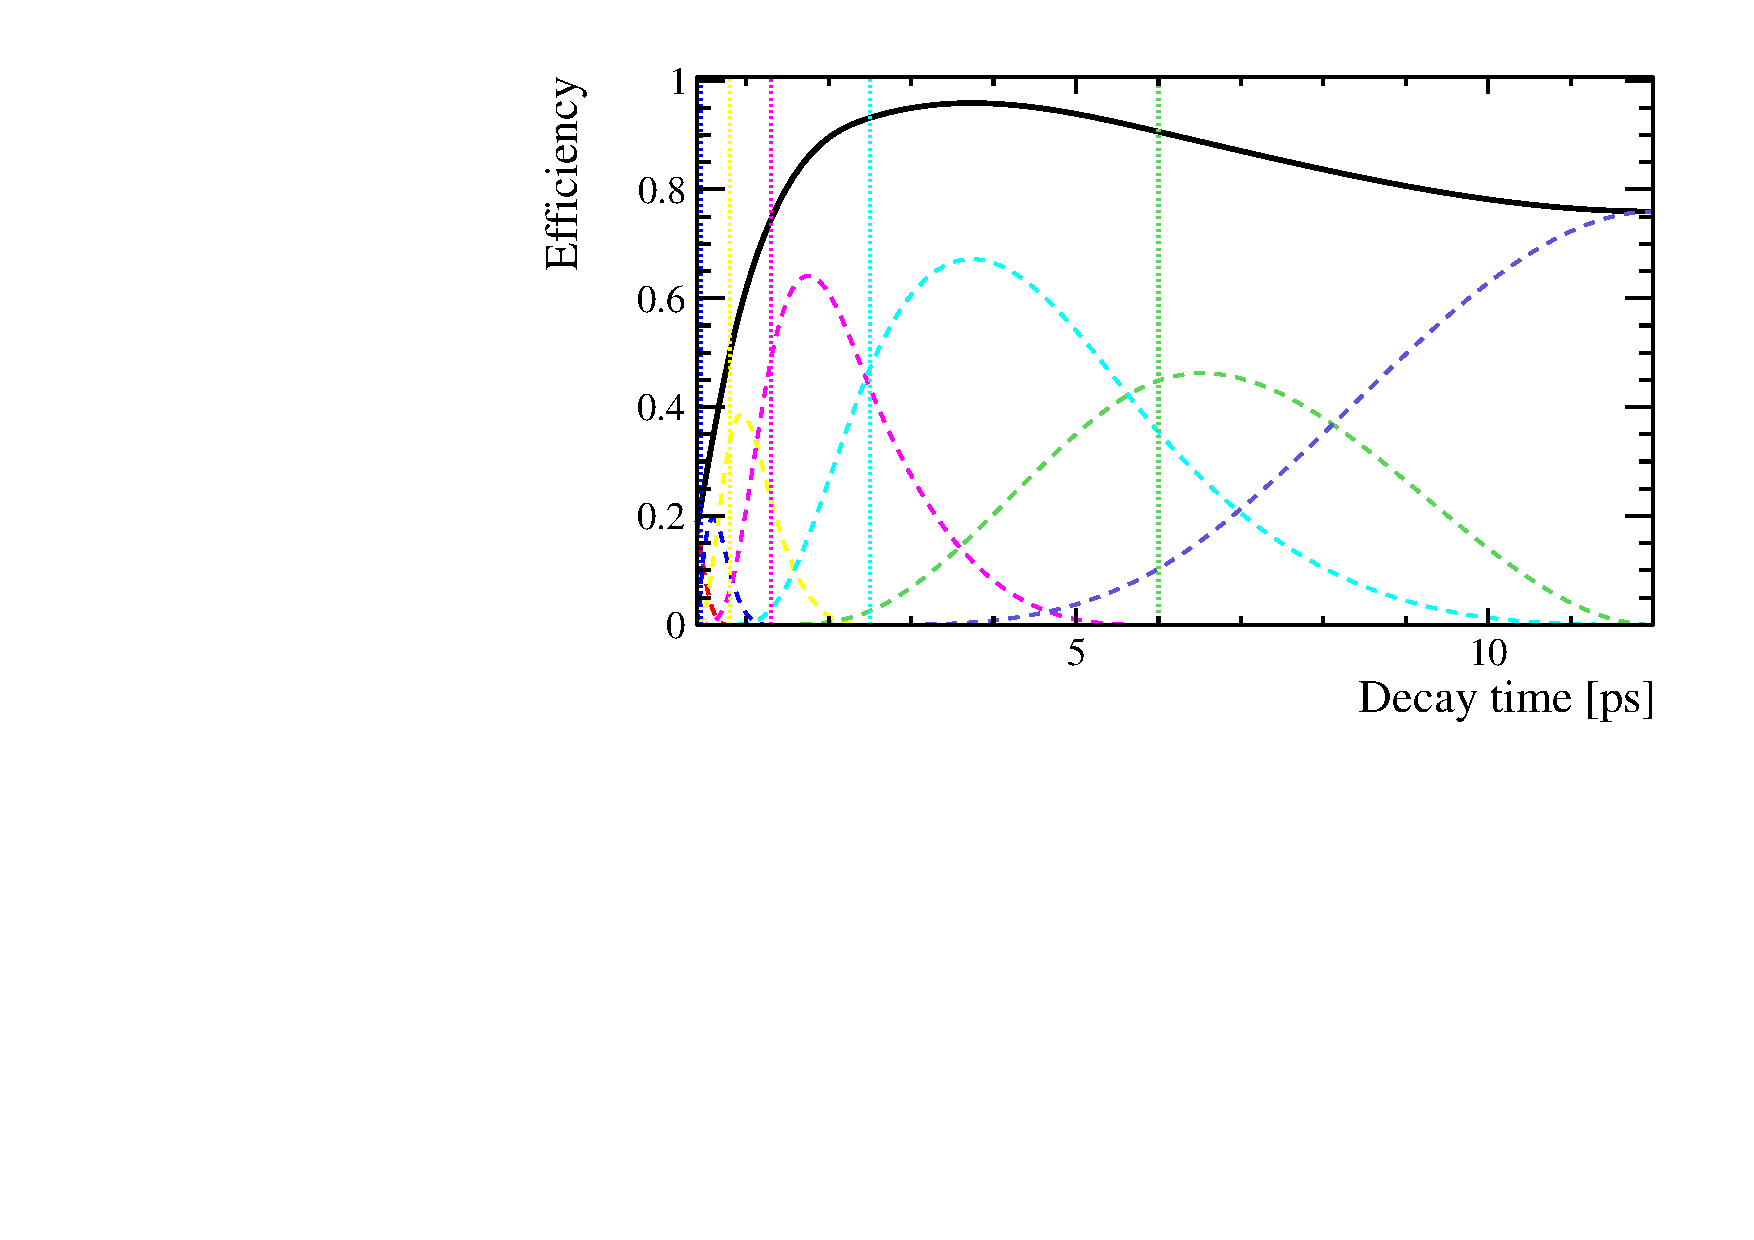
\includegraphics[width=0.7\textwidth]{10TimeFit/figs/Acceptance.pdf}
    \caption{Graphical representation of the acceptance for \BdToDpi decays.
    The dotted vertical lines represent the knot positions, the dashed lines show the underlying cubic polynomials, where the same colour is chosen for the associated knot and polynomial.}
    \label{fig:acceptance}
\end{figure}
\begin{table}[tbp]
	\centering
	\caption{Spline coefficients $v_i$ as obtained for the decay-time distribution on \BdToDpi.
	The coefficient $v_5$ is set to one to fix the overall normalisation.}
	\begin{tabular}{SS}
		\toprule
		{Parameter} & {Value} \\
		\midrule
		{$v_1$} 	& 0.187\pm0.004 \\
		{$v_2$} 	& 0.306\pm0.005 \\
		{$v_3$} 	& 0.557\pm0.005 \\
		{$v_4$} 	& 0.870\pm0.010 \\
        {$v_5$}     & 1.0 \\
		{$v_6$} 	& 0.880\pm0.023 \\
		{$v_7$} 	& 0.759\pm0.023 \\
		\bottomrule
	\end{tabular}
	\label{tab:acceptance}
\end{table}

\setmathfont[Scale=MatchUppercase]{XITS Math}
\subsection[head={Extraction of \CP observables},tocentry={Extraction of \CP observables}]{Extraction of $\symbfsf{\CP}$ observables}
\label{sec:ExtractCPobs}
\setmathfont{Tex Gyre Pagella Math}

The \CP parameters \Sf and \Sfbar are determined through a multi-dimensional unbinned maximum-likelihood fit to the \emph{sWeighted} (background-subtracted) distributions of \BdToDpi.
The PDF to describe the decay time $t$, the tags $\vec{d}=(d^{\text{\tiny OS}}, d^{\text{\tiny SS}})$ and the final state $F$ taking the values \f and \fbar given the mistags $\vec{\eta}=(\eta^{\text{\tiny OS}}, \eta^{\text{\tiny SS}})$ is defined by
\begin{equation}
\mathcal{P}(t, F, \vec{d}|\vec{\eta})\propto a(t)\left(P(t', F, \vec{d}|\vec{\eta})\otimes R(t'-t)\right)\label{eq:FinalDecayTimePDF}
\end{equation}
where $P(t', F, \vec{d}|\vec{\eta})$ describes the true decay time, $R(t'-t)$ is the resolution from \cref{sec:resolution} and $a(t)$ parametrises the acceptance described in \cref{sec:acceptance}.
Furthermore, the function $P(t', F, \vec{d}|\vec{\eta})$ corresponds to the decay rates from \crefrange{eq:DecRateB2Dmpip}{eq:DecRateBb2Dppim} taking into account the corrections from \cref{eq:decRateCorrectFT}.
Besides, production and detection asymmetry must be described.
These are defined as
\begin{equation}
A_{\text{P}}=\frac{\sigma(\Bzb)-\sigma(\Bz)}{\sigma(\Bzb)+\sigma(\Bz)}\hspace{0.5cm}\text{and}\hspace{0.5cm}A_{\text{D}}=\frac{\varepsilon(\,\f)-\varepsilon(\,\fbar)}{\varepsilon(\,\f)+\varepsilon(\,\fbar)}
\end{equation}
where $\varepsilon$ is the decay-time integrated reconstruction and selection efficiency for the final states \f and \fbar and $\sigma$ is the production cross-section for \Bz and \Bzb mesons.
Both asymmetries were determined to be at the percent level in independent measurements at the \lhc~\cite{Aaij:2017mso}.
As both are further known to be decay-time independent they can be described by modifying the expressions for the \CP coefficients from \cref{eq:decRateCorrectFT} further to
\begin{equation}
\begin{aligned}
\left(\Delta^--\Delta^+\right)\Sf&\to\left(\Delta^--A_{\text{P}}\,\Delta^+\right)(1+A_{\text{D}})\Sf\,,\\
\left(\Delta^--\Delta^+\right)\Cf&\to\left(\Delta^--A_{\text{P}}\,\Delta^+\right)(1+A_{\text{D}})\Cf\,.
\end{aligned}
\end{equation}
The same expressions also apply to \Sfbar and \Cfbar with the substitution $A_{\text{D}}\to -A_{\text{D}}$.

As explained in \cref{sec:taggingstrategy}, the parameters \Cf and \Cfbar are fixed to \num{1} and \num{-1}, due to the expected small value of $r$ (see \cref{sec:GammaInBd2Dpi}).
Moreover, since possible tagging efficiency asymmetries are measured in simulation to be compatible with zero, they are fixed to this value for the OS and SS taggers.
Possible systematic effects due to one of both assumptions are taken into account in \cref{ch:systeamticUncerts}.
Furthermore, the the \Bz lifetime and the oscillation frequency are constrained by means of a Gaussian function to $\tau=\SI{1.518\pm0.004}{\pico\second}$~\cite{PDG2018} and $\dm=\SI{0.5050\pm0.0023}{\per\pico\second}$~\cite{Aaij:2016fdk}.
Hence, the completely floating parameters in the fit are the \CP parameters \Sf and \Sfbar, the production and detection asymmetry, the calibration parameters of the OS and SS taggers and the acceptance parameters.
The fitted values for the parameters \Sf, \Sfbar, \dm, \DG, $A_{\text{P}}$ and $A_{\text{D}}$ are shown in \cref{tab:DecTimeProjection}.
Figure \ref{fig:DecTimeProjection} shows the projection of the PDF onto the decay-time distribution.
For the \CP parameters \Sf and \Sfbar, it is important to note that the given uncertainties are not purely statistical, but also include the systematic contributions from \dm and $\tau$ via the applied constraints.
Repeating the fit with \dm and $\tau$ fixed to the central values of the constraints, the central values for \Sf and \Sfbar stay unchanged, but the uncertainties decrease to \num{0.020}.
\begin{figure}[tbp]
    \centering
    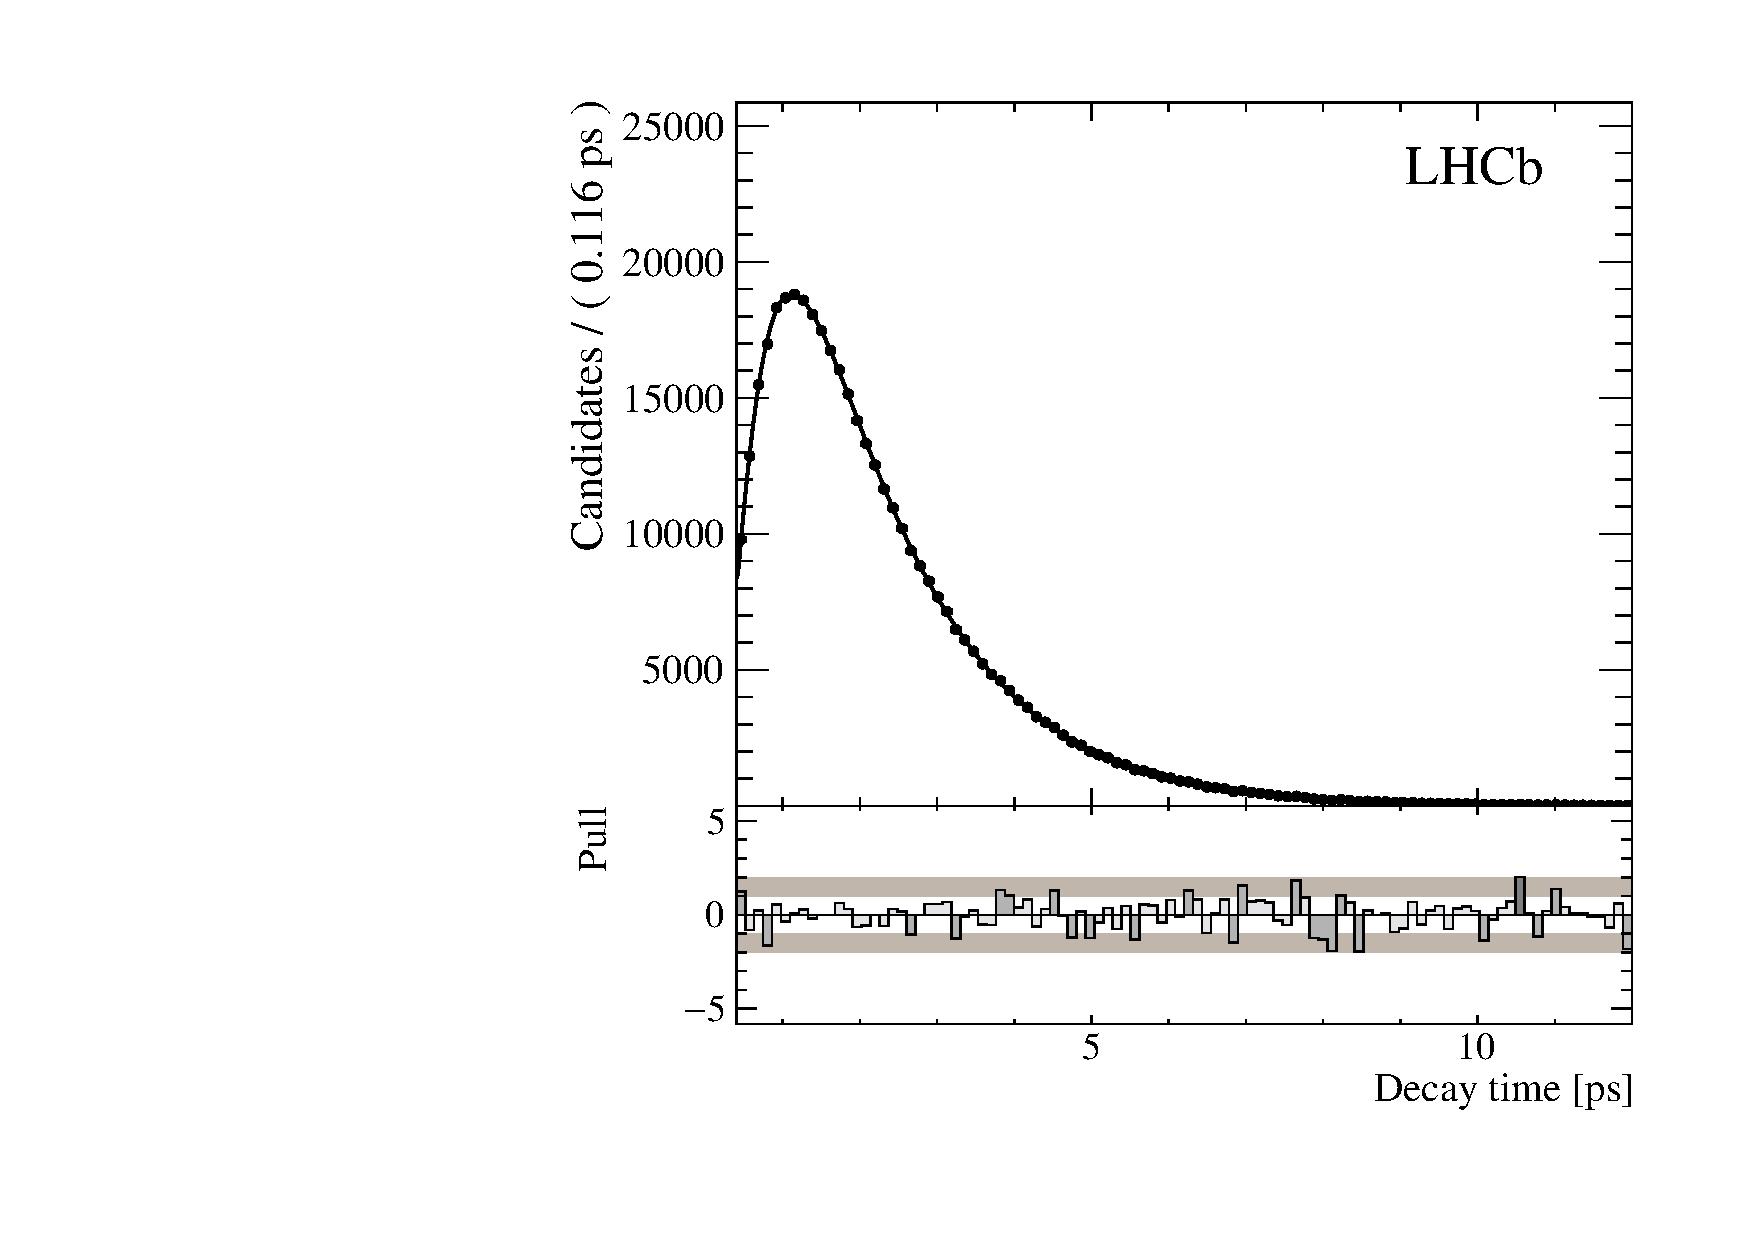
\includegraphics[width=0.7\textwidth]{10TimeFit/figs/BeautyTime_pull.pdf}
    \caption{Background-subtracted decay-time distribution of \BdToDpi candidates.
    The solid curve is the projection of the PDF, the black points represent the data.
    The lower histogram shows the distributions of pulls, \ie the difference of the binned data and the fitted PDF divided by the data uncertainty in each bin.}
    \label{fig:DecTimeProjection}
\end{figure}

\begin{table}[tbp]
	\centering
	\caption{Fit results for \Sf, \Sfbar, \dm, \DG, $A_{\text{P}}$ and $A_{\text{D}}$ from the nominal decay-time fit in \mbox{\BdToDpi}.
	The uncertainties on \Sf and \Sfbar are not purely statistical, but contain the systematic contributions from the constraints on \dm and $\tau$.}
	\begin{tabular}{Sr@{\,\( \pm \)\,}l@{\,}s[table-unit-alignment = left]}
		\toprule
		{Parameter} & \multicolumn{3}{c}{\kern -1.1cm Value}  \\
		\midrule
		{\Sf} 				& $0.058\hphantom{0}$ & $0.021$ \\
		{\Sfbar} 			& $0.038\hphantom{0}$ & $0.021$ \\
		{\dm} 				& $(0.5054$ & $0.0022)$ & \si{\per\pico\second} \\
		{$\tau$} 			& $(1.5180$ & $0.0040)$ & \si{\pico\second} \\
		{$A_{\text{P}}$} 	& $-0.0064$ & $0.0028$ \\
		{$A_{\text{D}}$} 	& $0.0086$ & $0.0019$ \\
		\bottomrule
	\end{tabular}
	\label{tab:DecTimeProjection}
\end{table}
In \cref{fig:AsymProjection}, the signal yield asymmetries given by
\begin{equation}
\begin{aligned}
A_{\CP}^{\,f}(t)\!=\!\frac{\Gamma\!\left(\Bz\!\to\Dm\pip\right)-\Gamma\!\left(\Bzb\!\to\Dm\pip\right)}{\Gamma\!\left(\Bz\!\to\Dm\pip\right)+\Gamma\!\left(\Bzb\!\to\Dm\pip\right)}\!\propto\!-\Sf\sin\!\left(\dm t\right)+\Cf\cos\!\left(\dm t\right)\,,\\
A_{\CP}^{\,\kern 1.5pt\overline{\kern -1.5pt f\kern 1.5pt}}(t)\!=\!\frac{\Gamma\!\left(\Bz\!\to\Dp\pim\right)-\Gamma\!\left(\Bzb\!\to\Dp\pim\right)}{\Gamma\!\left(\Bz\!\to\Dp\pim\right)+\Gamma\!\left(\Bzb\!\to\Dp\pim\right)}\!\propto\!-\Sfbar\sin\!\left(\dm t\right)+\Cfbar\cos\!\left(\dm t\right)\,,
\end{aligned}
\end{equation}
when neglecting the asymmetries from the flavour tagging and in the detection and production are shown.
Obviously, for these asymmetries values for \Sf and \Sfbar different from zero would show a shifted oscillation with respect to the cosine oscillation, which stems from the \Bz-\Bzb mixing.
However, such shift would only be a necessary but not sufficient condition for \CP violation as pointed out in \cref{eq:condForIntCPV}:
in the case that \CP violation occurs in the decay \BdToDpi the shift must be different for the asymmetries $A_{\CP}^{\,f}(t)$ and $\smash{A_{\CP}^{\,\kern 1.5pt\overline{\kern -1.5pt f\kern 1.5pt}}(t)}$.
Unfortunately, the values for \Sf and \Sfbar are small, so that these asymmetries are mainly dominated by the cosine term and therefore even a shift is barely visible.
A better alternative, not suffering from this discrepancies in magnitude between $\smash{\Sf/\Sfbar}$ and $\Cf/\Cfbar$, are the signal yield asymmetries between candidates tagged as \Bz and \Bzb split according to the favoured (F) $\bquarkbar\!\to\cquarkbar\uquark\dquarkbar$ and the suppressed (S) $\bquarkbar\!\to\uquarkbar\cquark\dquarkbar$ transitions.
Neglecting again asymmetries in the flavour tagging and in the detection and production these can be expressed as
\begin{equation}
\begin{aligned}
A_{\text{F}}(t)&=\frac{\Gamma\!\left(\Bz\!\to\Dm\pip\right)-\Gamma\!\left(\Bzb\!\to\Dp\pim\right)}{\Gamma\!\left(\Bz\!\to\Dm\pip\right)+\Gamma\!\left(\Bzb\!\to\Dp\pim\right)}\propto-\left(\Sf+\Sfbar\right)\sin\!\left(\dm t\right)\,,\\
A_{\text{S}}(t)&=\frac{\Gamma\!\left(\Bzb\!\to\Dm\pip\right)-\Gamma\!\left(\Bz\!\to\Dp\pim\right)}{\Gamma\!\left(\Bzb\!\to\Dm\pip\right)+\Gamma\!\left(\Bz\!\to\Dp\pim\right)}\propto\left(\Sf+\Sfbar\right)\sin\!\left(\dm t\right)\,.\label{eq:AsymeSuppFav}
\end{aligned}
\end{equation}
Apparently, the cosine terms in the numerator vanishes, so that in case of no \mbox{\CP violation}, \ie $\Sf=\Sfbar$, the asymmetries vanish.
However, as shown in \cref{fig:AsymProjection} an oscillation indicating \CP violation can be seen.
Yet, neglecting the contributing experimental asymmetries in \cref{eq:AsymeSuppFav} oversimplified the expressions, as indicated by an alternative fit under the asumption of no \CP violation: the resulting fit projection is not flat, but also shows an oscillating structure from contributions of the asymmetries in the numerator on the one hand and from sine and cosine contributions arising in the denominator of $A_{\text{F}}(t)$ and $A_{\text{S}}(t)$ on the other hand.
The difference between these two fits yields a significance of $2.7\sigma$ for \mbox{\CP violation} according to Wilk's theorem~\cite{wilks1938}.
\begin{figure}[tbp]
    \centering
    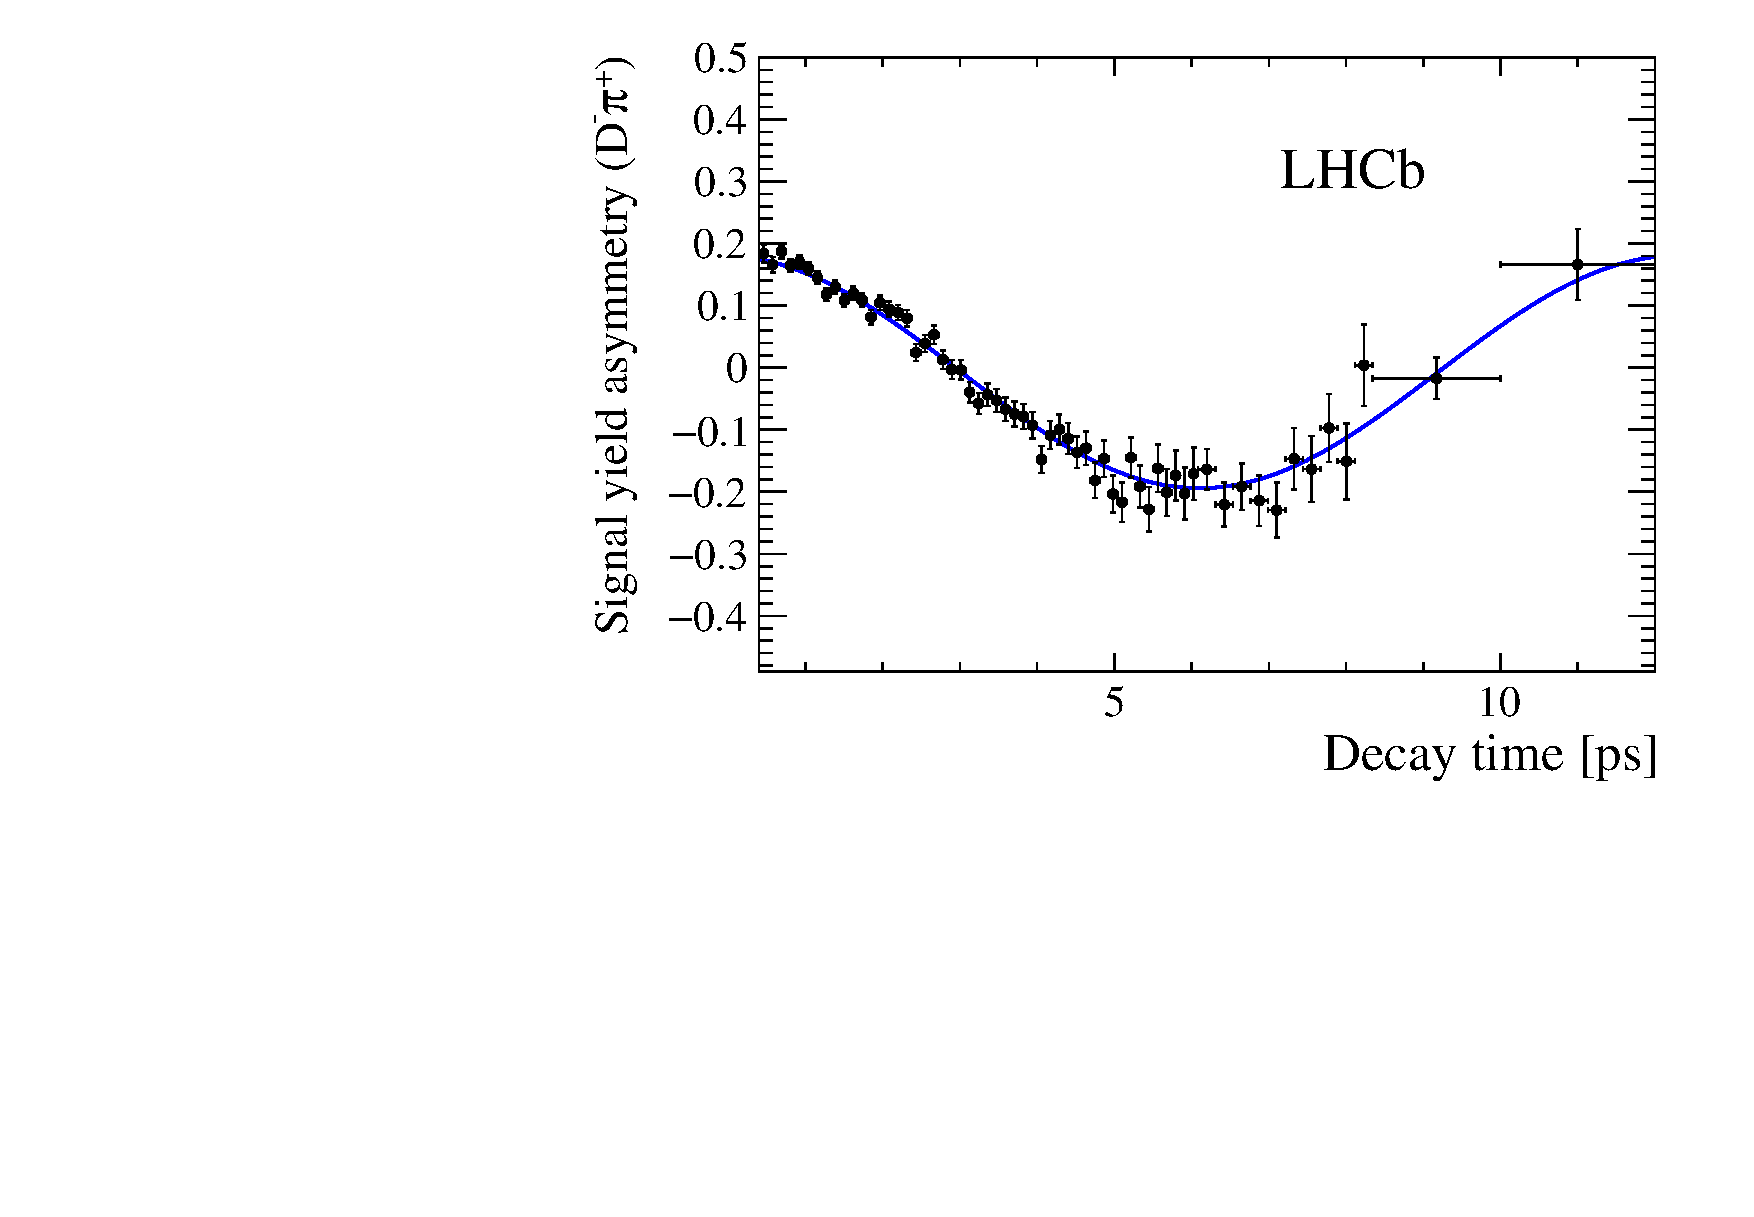
\includegraphics[width=0.48\textwidth]{10TimeFit/figs/Asym_f.pdf}
    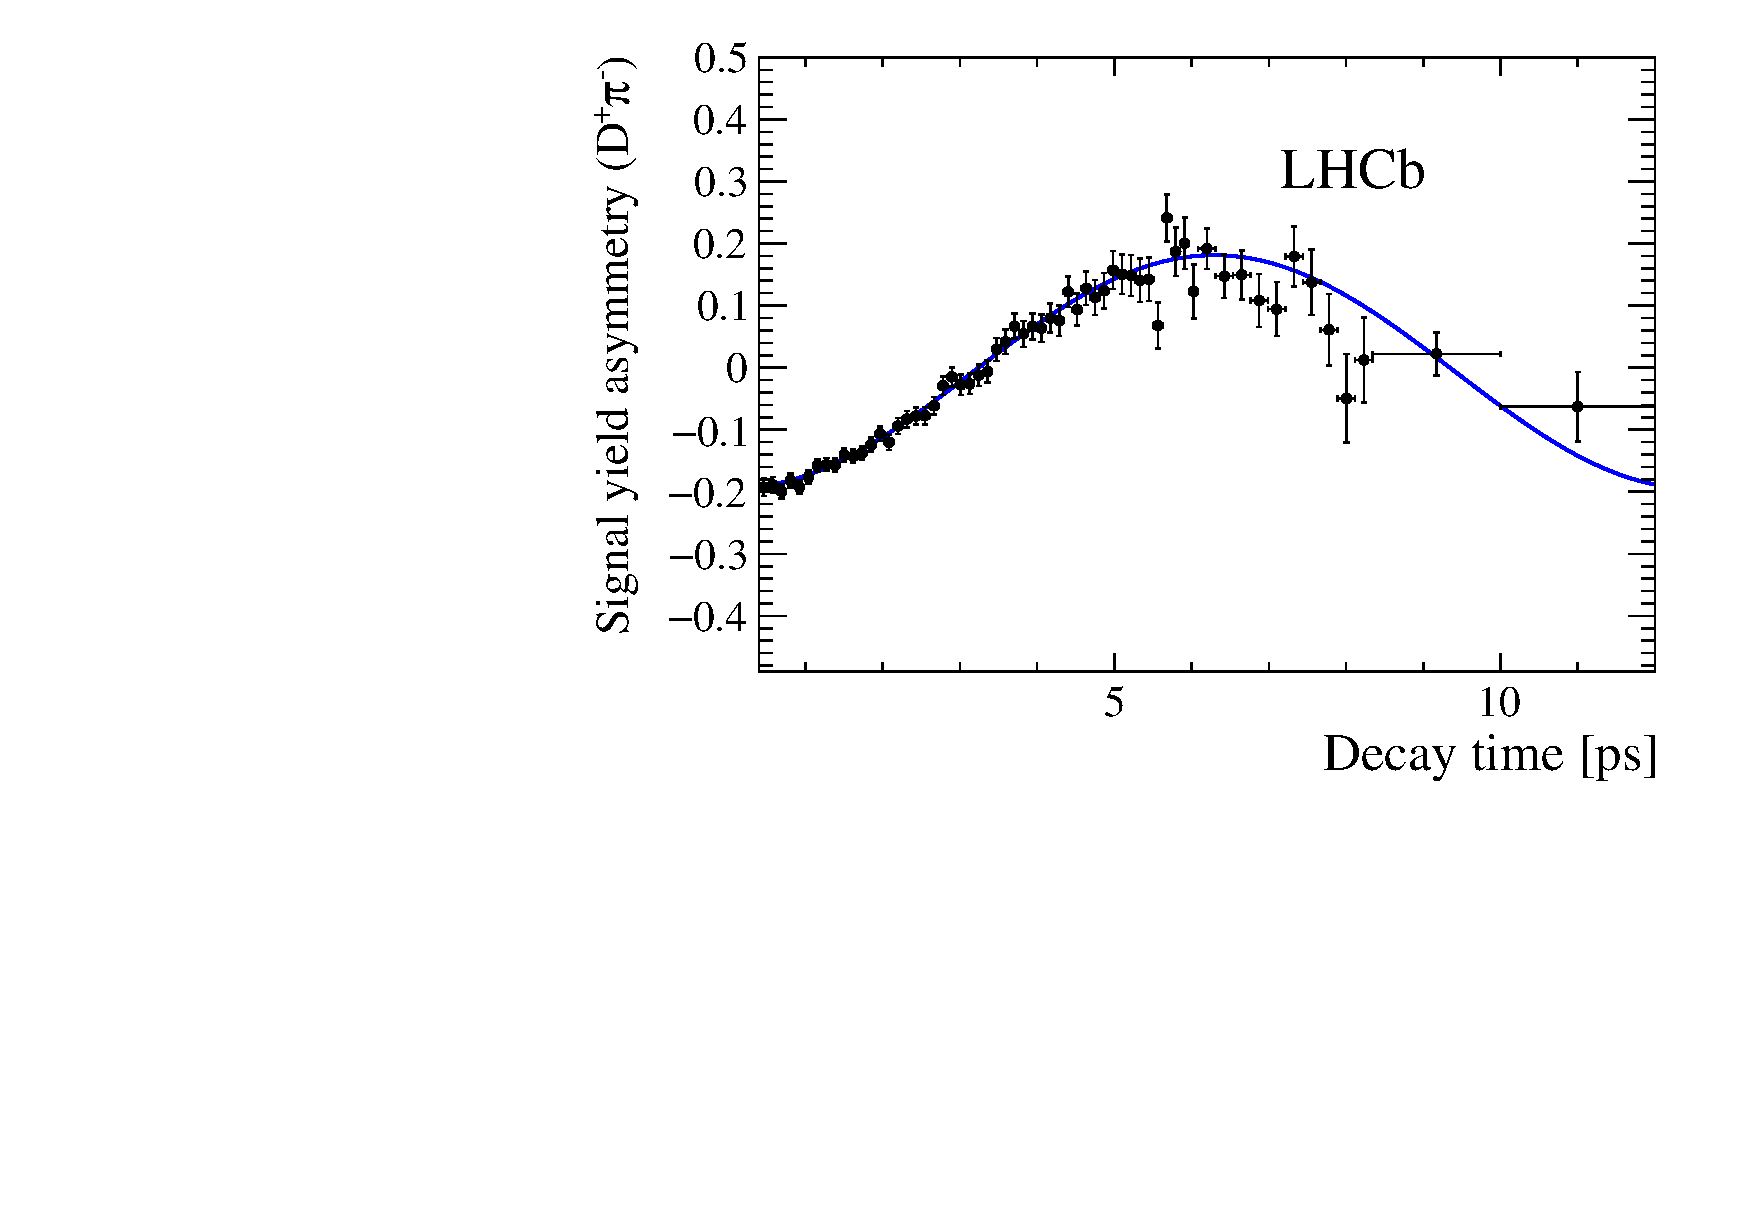
\includegraphics[width=0.48\textwidth]{10TimeFit/figs/Asym_fbar.pdf}\\
    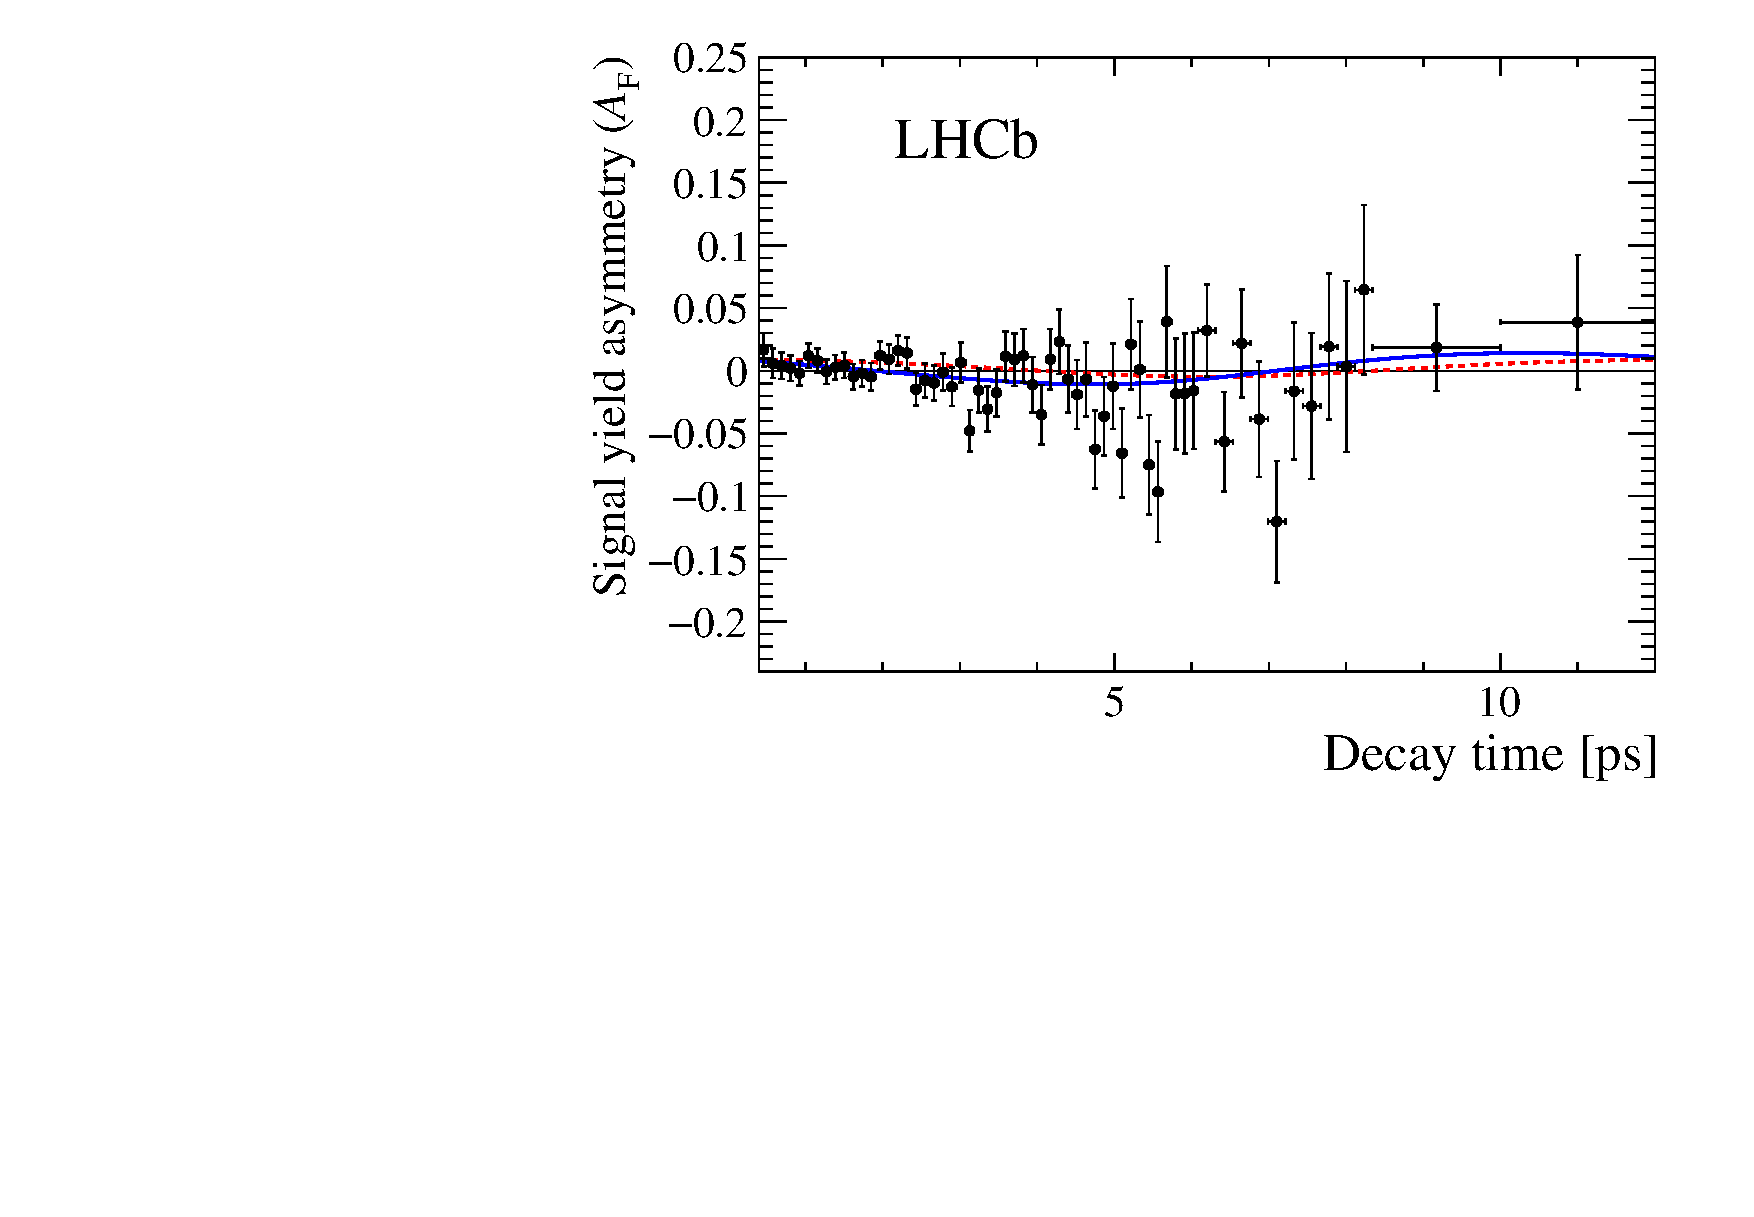
\includegraphics[width=0.48\textwidth]{10TimeFit/figs/Asym_favour.pdf}
    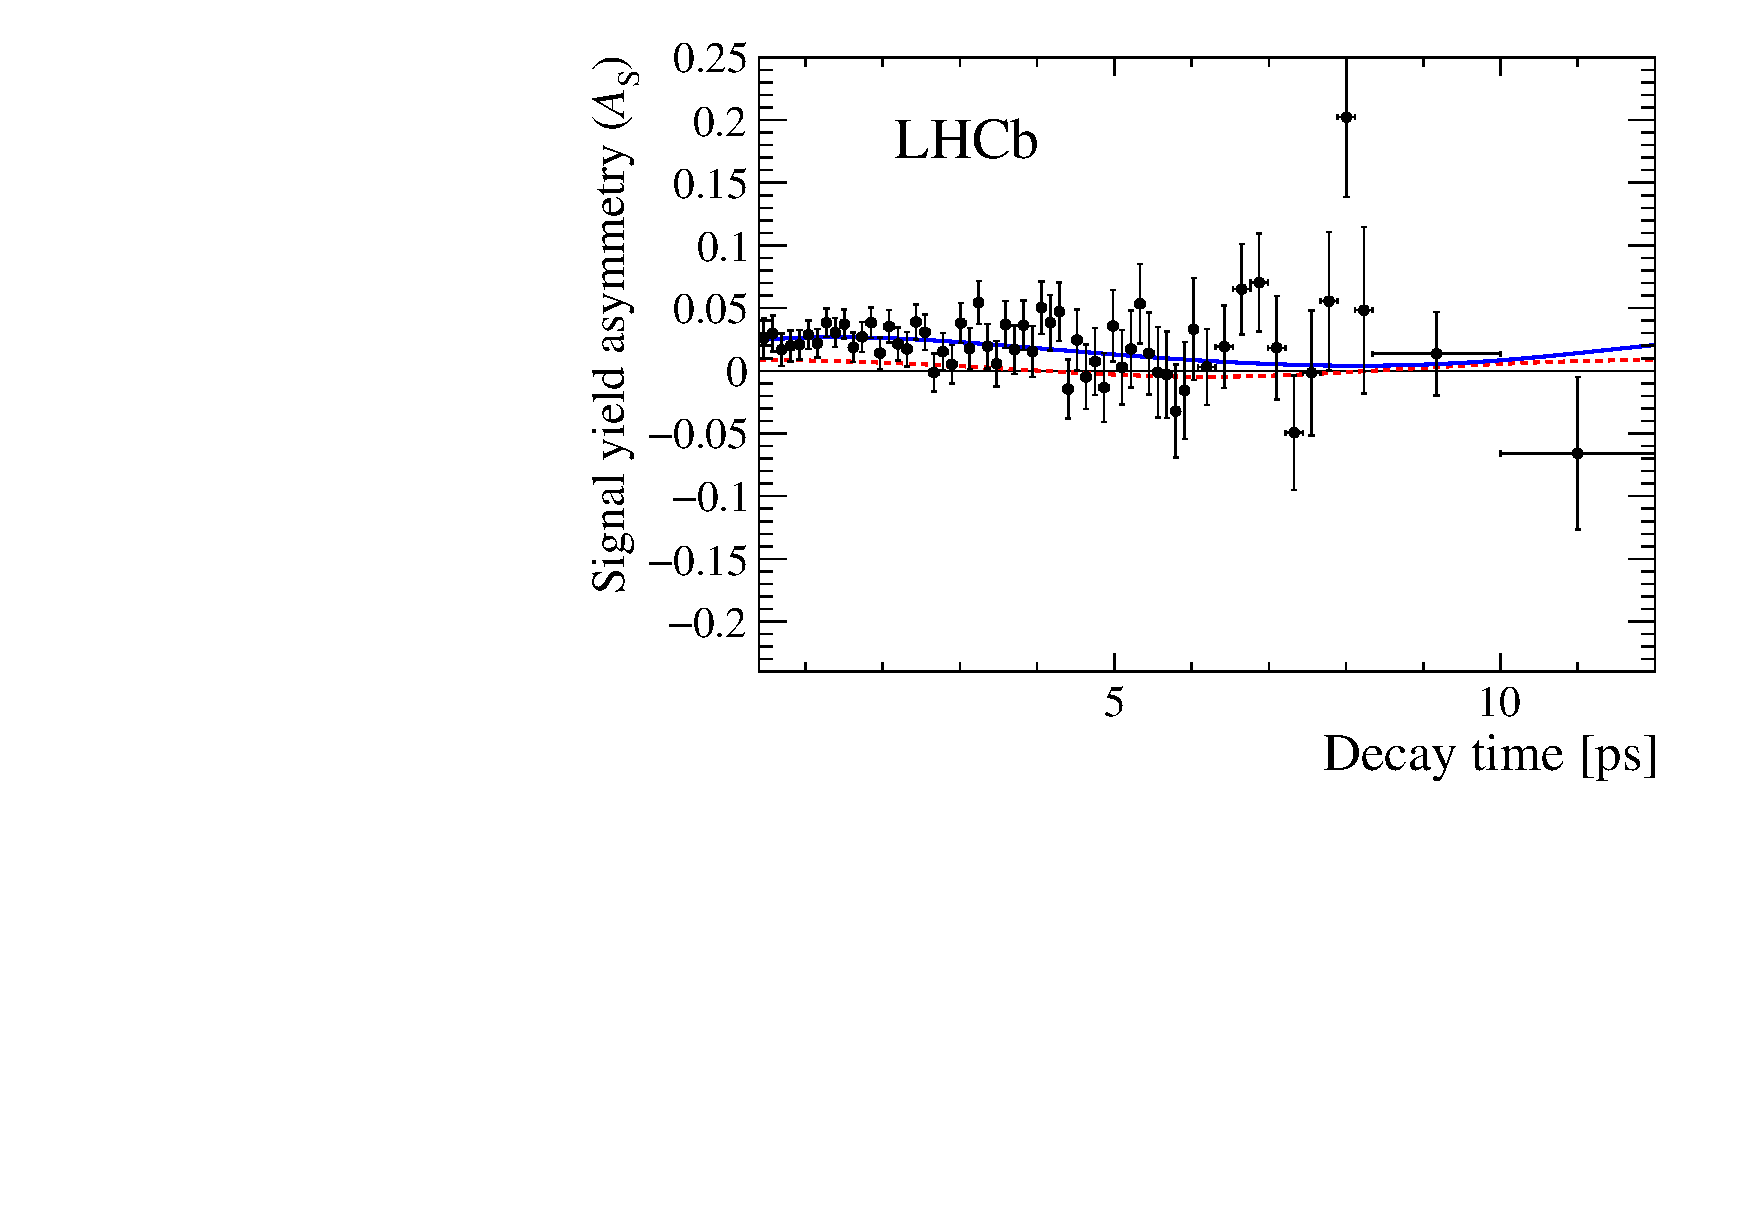
\includegraphics[width=0.48\textwidth]{10TimeFit/figs/Asym_suppress.pdf}
    \caption{Distributions of the decay-time dependent signal yield asymmetry for the \Dm\pip (top left) and the \Dp\pim (top right) finalstate and of the decay-time dependent signal yield asymmetry for the favoured (bottom left) and the suppressed (bottom right) transitions as defined in \cref{eq:AsymeSuppFav}.
    The blue solid curve is the projection of the fitted PDF from the nominal fit, the red dotted curve in the lower plots shows the projection of a second fit under the assumption of no \CP violation.}
    \label{fig:AsymProjection}
\end{figure}

Using the results of the fitted calibration parameters (the results themselves are discussed in \cref{sec:decTimeFitVal}) and the fitted tagging efficiencies of $\varepsilon_{\text{tag}}^{\text{\tiny OS}}=\SI{43.24\pm0.07}{\percent}$ and $\varepsilon_{\text{tag}}^{\text{\tiny SS}}=\SI{93.05\pm0.04}{\percent}$, the tagging performances in the sample can be computed as shown in \cref{eq:perEenttaggingpower}.
The average dilution  as defined in \cref{eq:avgDilution} is \SI{9.53\pm0.03}{\percent} and \SI{2.789\pm0.009}{\percent} for the OS and SS taggers, respectively.
This leads to an overall average dilution of \SI{6.55\pm0.02}{\percent}.
Including the untagged candidates, which were removed in \cref{ch:massfit}, the total effective tagging efficiency is calculated to be \SI{5.59\pm0.01}{\percent}.

\section{Fit validation}
\label{sec:decTimeFitVal}

To validate the decay-time fit, first the fitted nuisance parameters like the production and detection asymmetry and the flavour tagging calibration parameters are compared to reference values.
The results of $A_{\text{P}}=\SI{-0.64\pm0.28}{\percent}$ and $A_{\text{D}}=\SI{0.86\pm0.19}{\percent}$ are well in agreement with the values from an independent \lhcb measurement~\cite{Aaij:2017mso}, which \eg range from \SIrange{-1.43\pm0.86}{-0.56\pm0.30}{\percent} for measurements of the production asymmetry at centre-of-mass energies of \num{7} and \SI{8}{\tera\electronvolt} in the decay channels $\Bz\!\to\jpsi\Kstarz$ and $\Bs\!\to\Dsm\pip$.
The obtained calibration parameters are compared to those computed on the control channels $\Bu\!\to\Dz\pip$ and $\Bz\!\to\jpsi\Kstarz$ for the OS and SS, respectively.
In \cref{tab:taggingCalibCompare}, the parameters from the decay-time fit in \BdToDpi are listed and the deviation of each parameter to the calibrations given in \cref{tab:CalibSS} and \cref{tab:CalibOS} are calculated.
The largest deviation can be found for $\Delta p_{3}^{\text{\tiny OS}}$ and $\Delta p_{4}^{\text{\tiny OS}}$ being larger than two standard deviations.
Additionally, taking into account the correlations between the parameters an overall discrepancy is calculated yielding $0.91\sigma$ for the OS and $0.29\sigma$ for the SS taggers demonstrating that the results of flavour tagging calibrations are quite similar despite the not given portability.
\begin{table}[tbp]
	\centering
	\caption{Calibration parameters obtained in the decay-time fit in \BdToDpi.
	The deviations are calculated with respect to the calibration parameters derived from the control modes $\Bu\!\to\Dz\pip$ (\cref{tab:CalibOS}) and $\Bz\!\to\jpsi\Kstarz$ (\cref{tab:CalibSS}).}
	\begin{tabular}{c|S[table-format=2.3,table-figures-uncertainty=1]S[table-format=1.2]|S[table-format=2.3,table-figures-uncertainty=1]S[table-format=1.2]}
		\toprule
		 & \multicolumn{2}{c|}{OS} & \multicolumn{2}{c}{SS}  \\
		\midrule
		{Parameter} & {Value} & {Deviation} & {Value} & {Deviation} \\
		\midrule
		{$p_0$} 		& -0.152\pm0.021 	& -0.56 & -0.041\pm0.021 & 0.80 \\
		{$p_1$} 		& -0.035\pm0.024 	& -0.89 & -0.012\pm0.022 & 0.22 \\
		{$p_2$} 		& -0.007\pm0.009 	& -0.33 & {-} 			 & {-} \\
		{$p_3$} 		& -0.32\pm0.11 		& 0.90  & {-}			 & {-} \\
		{$p_4$} 		& -0.47\pm0.49 		& 0.57  & {-}			 & {-} \\
		{$\Delta p_0$} 	& -0.079\pm0.049 	& 0.81  & -0.085\pm0.044 & -1.25 \\
		{$\Delta p_1$} 	& 0.140\pm0.036 	& 1.72  & 0.042\pm0.033  & 0.11 \\
		{$\Delta p_2$} 	& -0.024\pm0.013 	& -0.19 & {-} 			 & {-} \\
		{$\Delta p_3$} 	& -0.26\pm0.16 		& -2.66 & {-} 			 & {-} \\
		{$\Delta p_4$} 	& -0.52\pm0.71 		& -2.11 & {-} 			 & {-} \\
		\bottomrule
	\end{tabular}
	\label{tab:taggingCalibCompare}
\end{table}

In a second step, the two-dimensional contour plots for the \CP parameters \Sf and \Sfbar and for the detection and production asymmetries are checked.
As shown in \cref{fig:corrPlots} both do not show any unexpected behaviour, indicating that the corresponding uncertainties are well understood.
\begin{figure}[tbp]
    \centering
    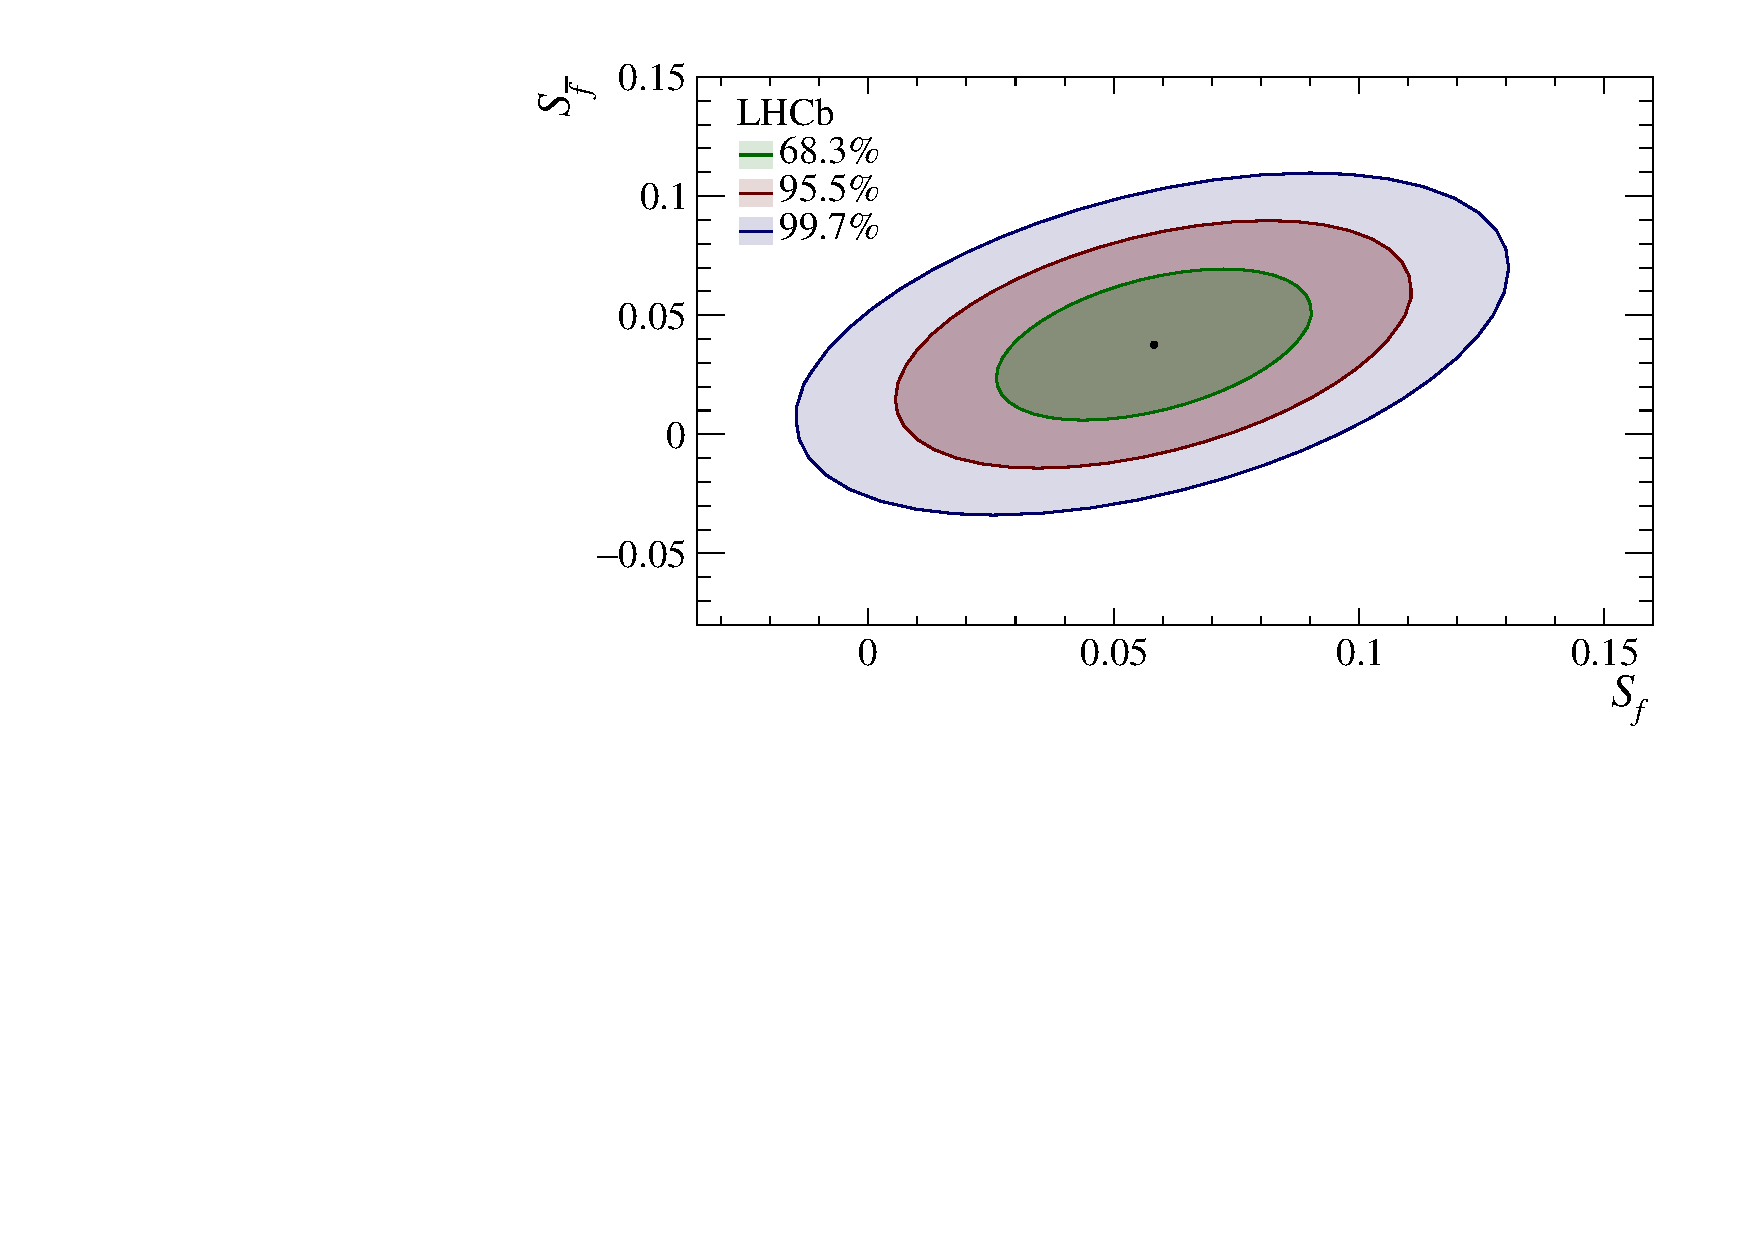
\includegraphics[width=0.48\textwidth]{10TimeFit/figs/SfvsSfbar.pdf}
    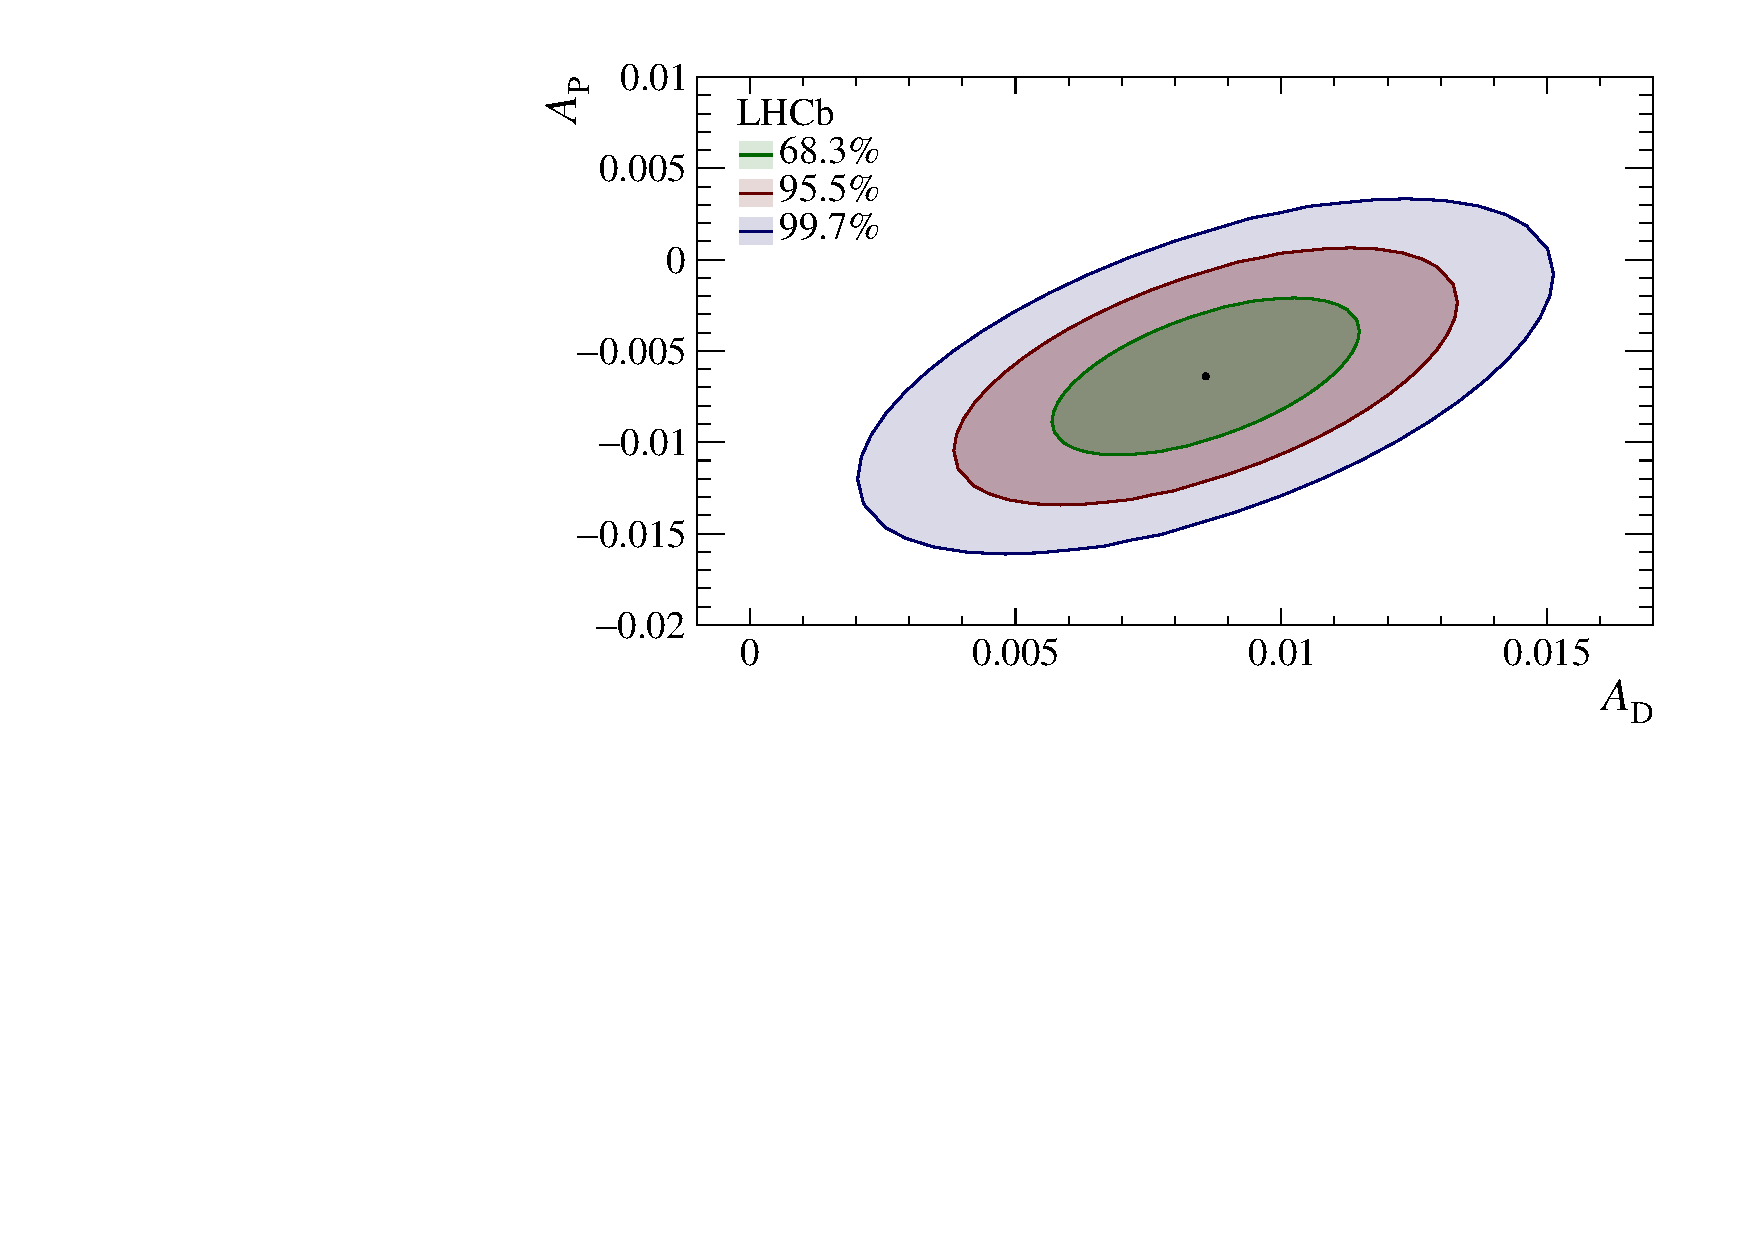
\includegraphics[width=0.48\textwidth]{10TimeFit/figs/ApvsAd.pdf}
    \caption{Contour plot for (\Sf, \Sfbar) (left) and ($A_{\text{P}}$, $A_{\text{D}}$) (right) showing the one, two and three sigma contours.
    The uncertainties include the full statistical uncertaintiy and the systematic uncertainty due to the constraints on \dm and $\tau$.}
    \label{fig:corrPlots}
\end{figure}

\subsection{Validation of link function for mistags}
\label{sec:ValLinkFunction}

As mentioned before, the handling of candidates with a mistag close to \num{0.5} is important, both in case of a calibration with parameters constrained by means of a Gaussian function and completely floating calibration parameters, to guarantee a stable and unbiased decay-time fit.
Therefore, the two scenarios presented additionally to the nominal scenario in \cref{sec:CombAndCalib} are tested using pseudoexperiments.

In each study presented below, \num{1000} pseudoexperiments are generated according to the PDF from \cref{eq:FinalDecayTimePDF}.
To simplify the used model and reduce the number of parameters, the flavour tagging calibration functions are reduced to linear models as \emph{basis functions} (see \cref{eq:linCalib}) and the identity as \emph{link function}.
The calibration parameters used for the generation are obtained from a linear calibration with the identity as \emph{link function} on the control channels $\Bu\!\to\Dz\pip$ and $\Bz\!\to\jpsi\Kstarz$.
It should be noted that the calibration for the OS taggers is shifting the estimated mistags to higher values, \ie $p_1^{\text{\tiny OS}}>1$, while the calibration for the SS taggers shows the opposite, \ie $p_1^{\text{\tiny SS}}<1$, behaviour.
Furthermore, the calibration function is implemented such that the mistag probability $\omega$ is not defined outside the range $[0, 0.5]$, \ie if the mistag probability exceeds \num{0.5}, the tag-decision is set to $d=0$ and the corresponding mistag to $\omega=0.5$.
For all studies presented in the following, the pull distributions of the floating parameters are checked, where the pull is defined as the fitted value minus the value used in the generation of the simulated sample divided by the uncertainty on the fitted value.
The pull distributions obtained from each set of pseudoexperiments are then fitted with a Gaussian function in order to determine the mean and width.
A deviation of more than one standard deviation of the mean value from zero indicates a possible bias, while a deviation of more than three standard deviations is interpreted as a clear bias.
These generated samples are then fitted with different approaches:
\begin{itemize}
	\item In the first approach,the tag decision is flipped in case the mistag probability $\omega'$ exceeds \num{0.5} and the mistag probability is calculated as $\omega=1-\omega'$.
	In the fit, the calibration parameters are constrained by means of a Gaussian function. This leads to biased calibration parameters for the OS algorithm.
	To understand if a possible bias on \Sf and \Sfbar is just \enquote{absorbed} by the calibration parameters, the same samples are also fitted with the calibration parameters fixed.
	In this case, the \CP parameters show a small deviation of $2\sigma$ and $1.3\sigma$ for \Sf and \Sfbar, respectively.
	\item To further understand if this small deviation is just a fluctuation or a real bias, two possible sources of the bias are investigated:
	in a first study the tagging asymmetry parameters $\Delta p_i^{\text{\tiny OS}}$ are artificially increased \ie the parameters are increased in both steps during generation and fitting.
    In a second study the tagging asymmetry parameters $\Delta p_i^{\text{\tiny OS}}$ are reduced to their nominal values but instead the parameter $p_1^{\text{\tiny OS}}$ is increased.
	In the fit, the tag decision is flipped in both studies if the mistag probability $\omega'$ exceeds \num{0.5} and the mistag probability is calculated as $\omega=1-\omega'$.
	To ensure that a possible bias is not \enquote{absorbed} by the calibration parameters, the calibration parameters are fixed in the fit .
	The resulting pull distributions for \Sf and \Sfbar are shown in \cref{fig:linkFunctionValid}.
	One can see that in case of the increased flavour tagging asymmetry parameters, the \CP parameters are clearly biased by more than ten standard deviations, while the result is unbiased in case of the enlarged $p_1^{\text{\tiny OS}}$ parameter.
	\begin{figure}[tbp]
    \centering
    	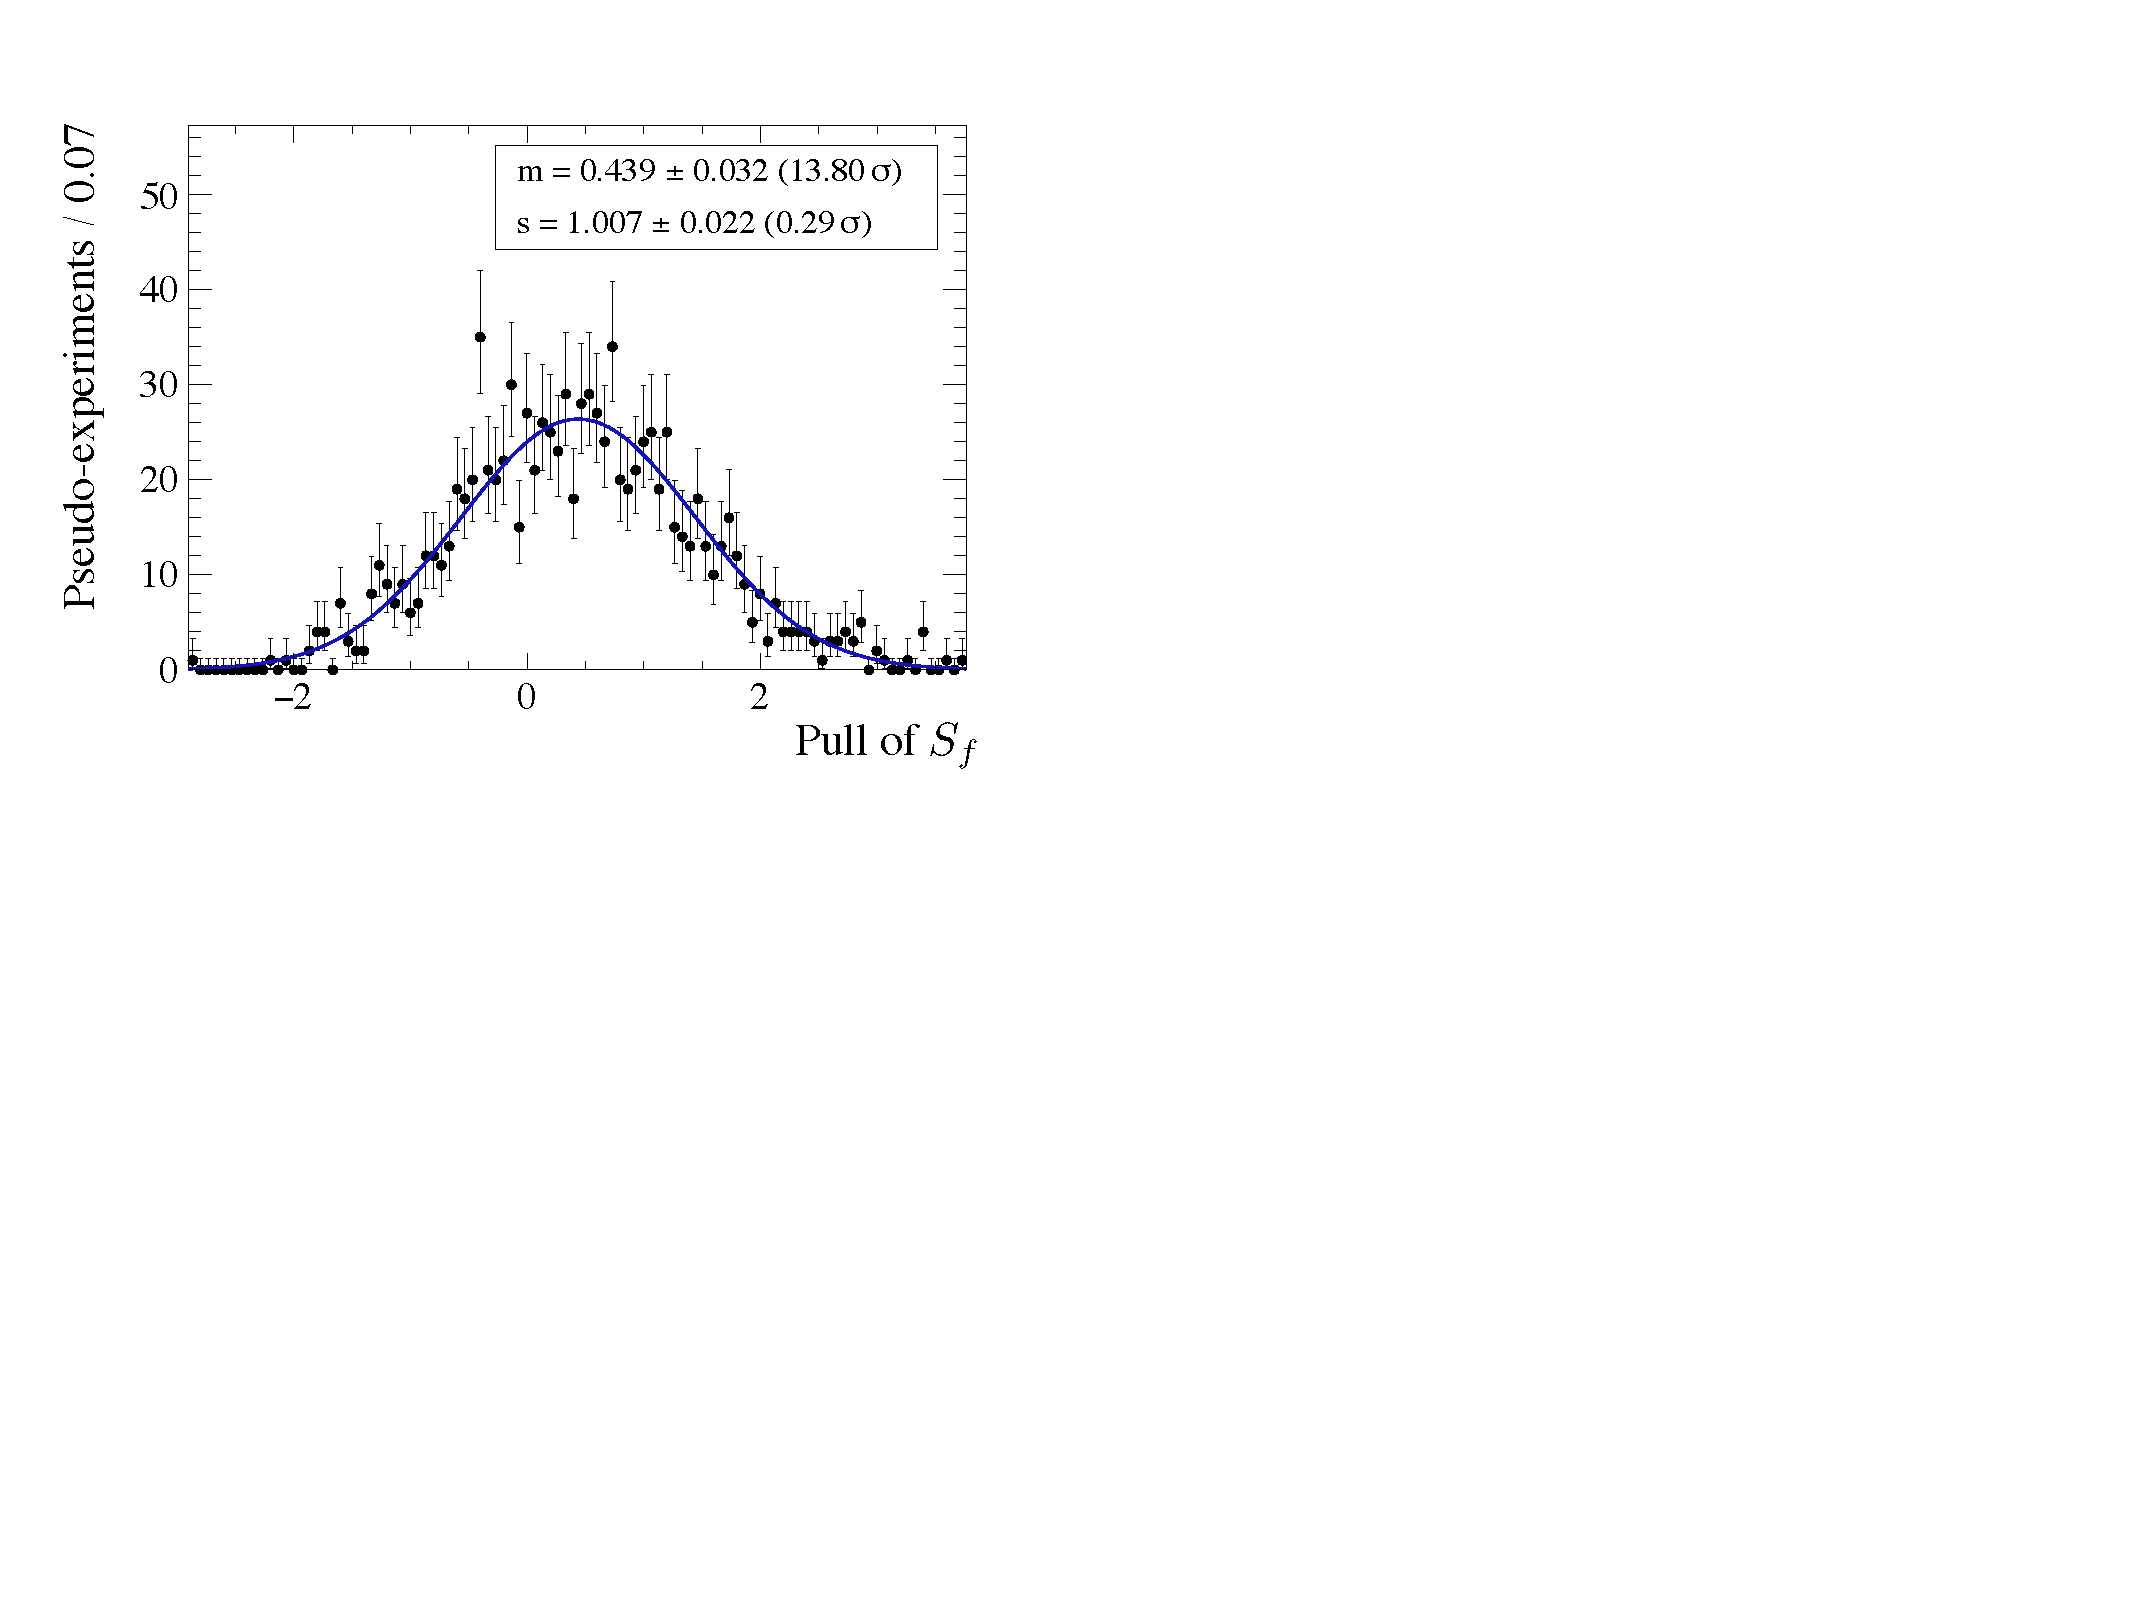
\includegraphics[width=0.48\textwidth]{10TimeFit/figs/Sf_pull_LinkValid_asym.pdf}
    	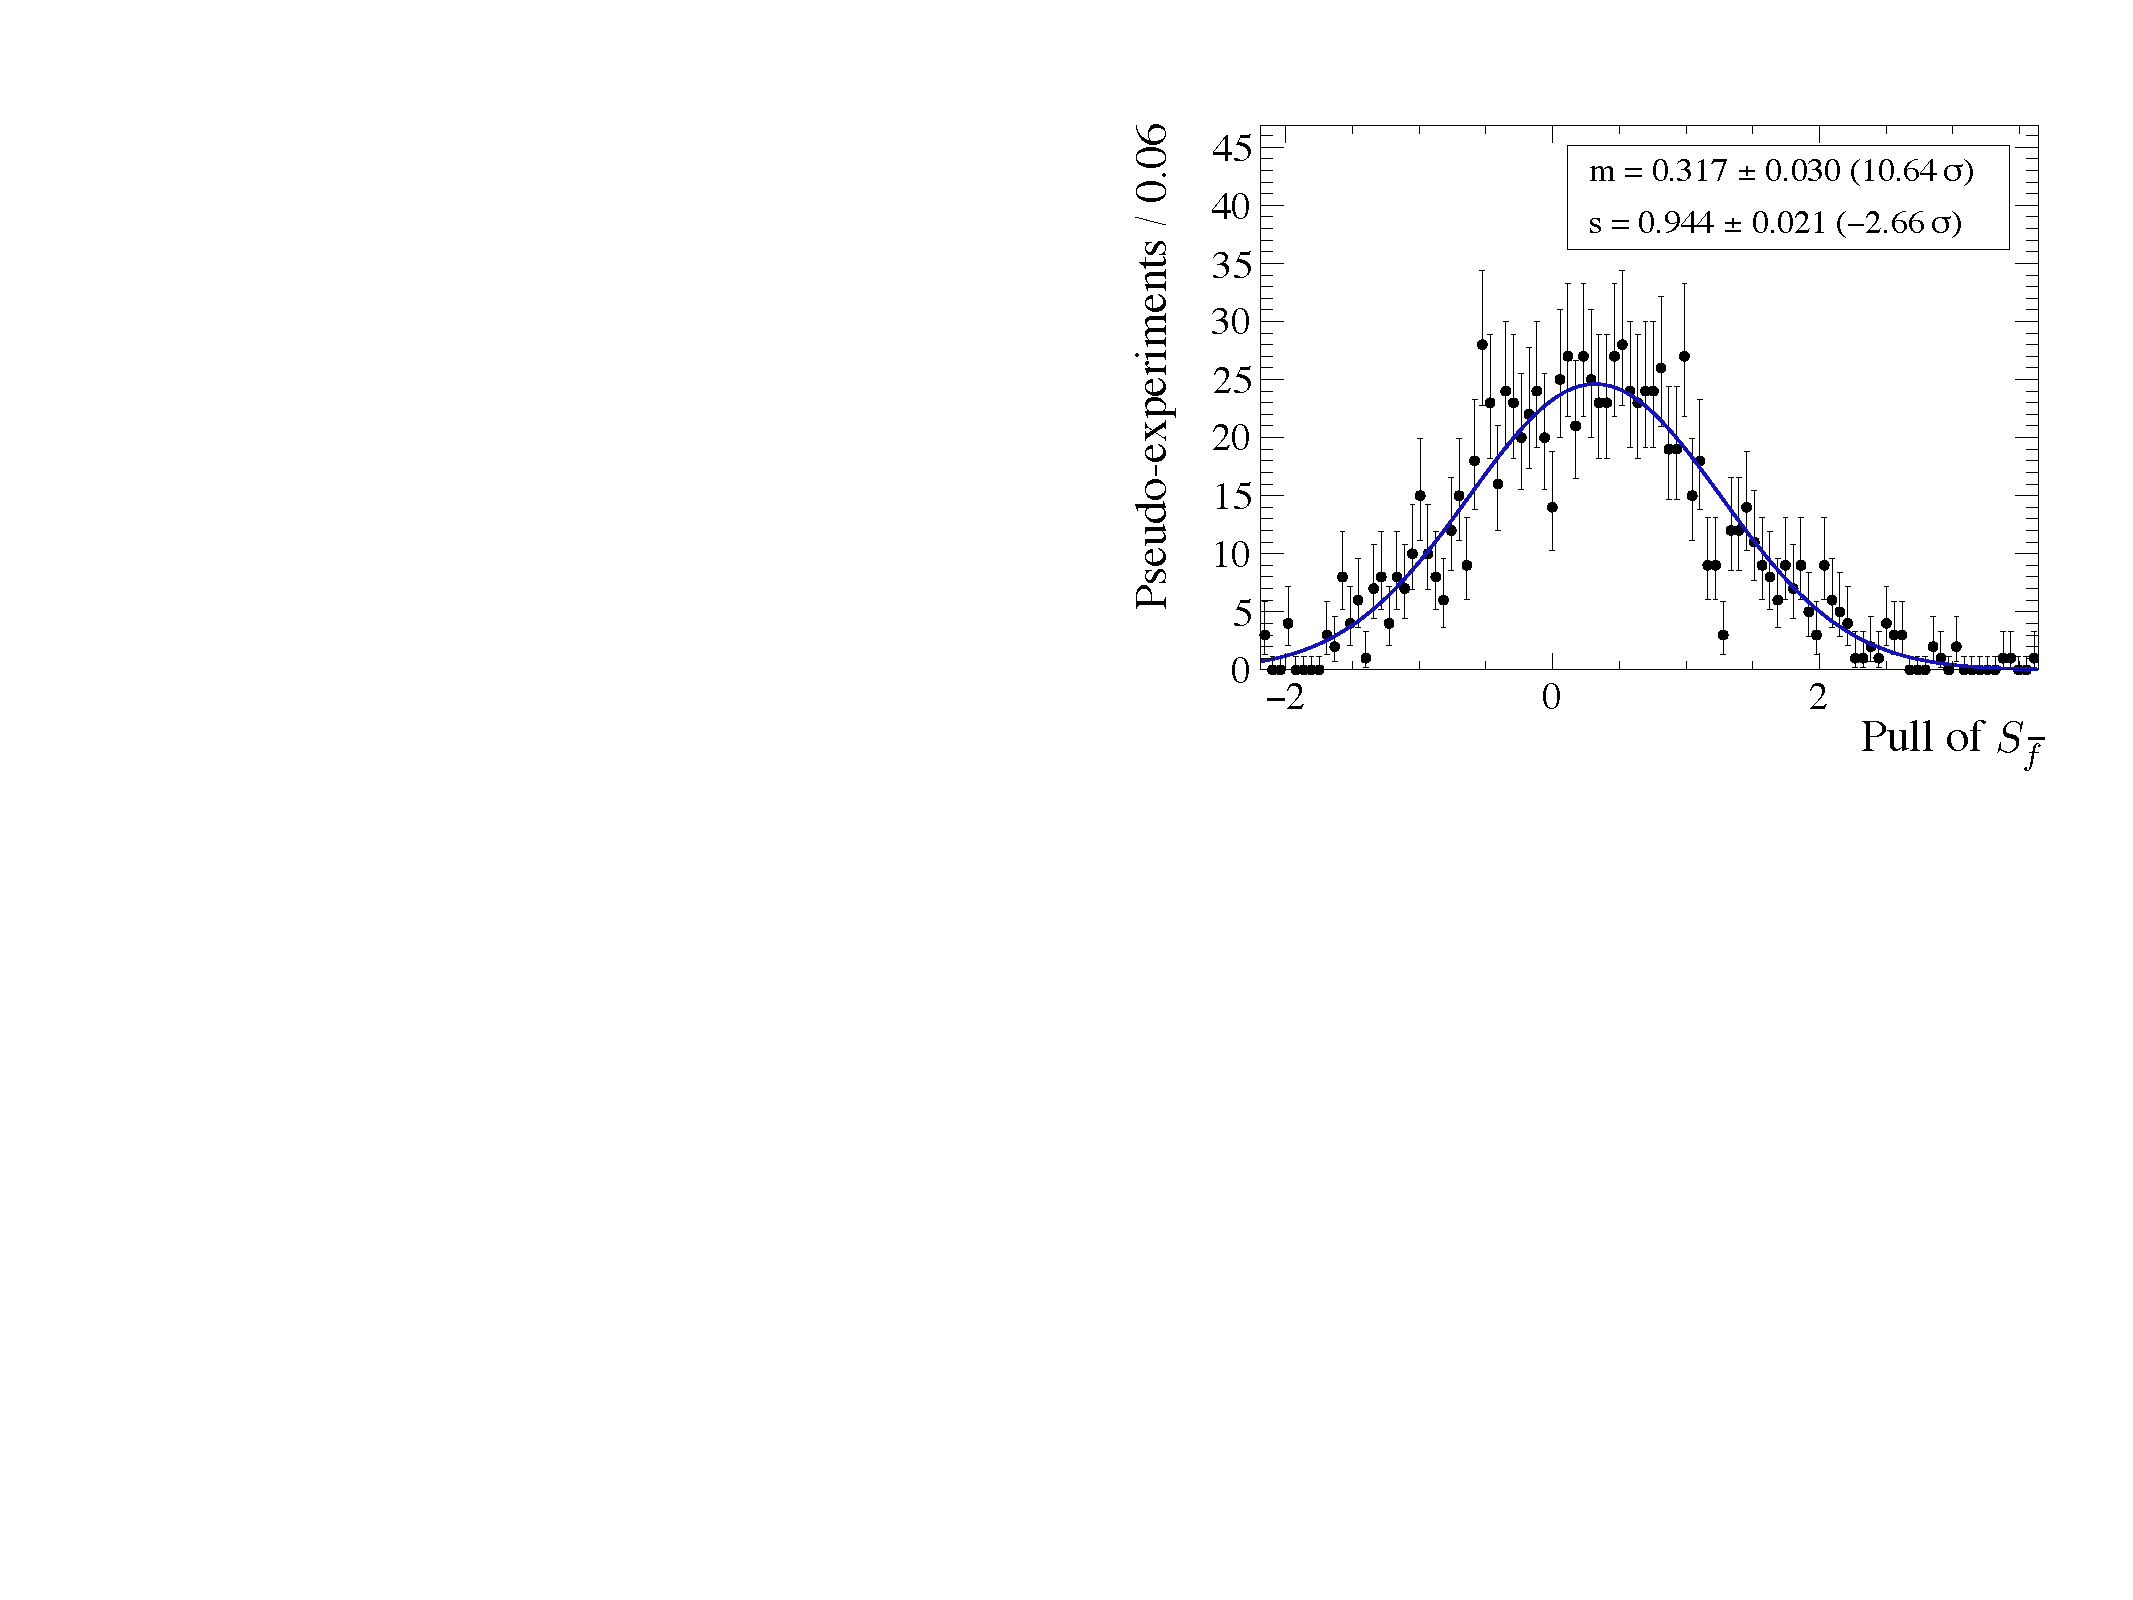
\includegraphics[width=0.48\textwidth]{10TimeFit/figs/Sfbar_pull_LinkValid_asym.pdf}\\
    	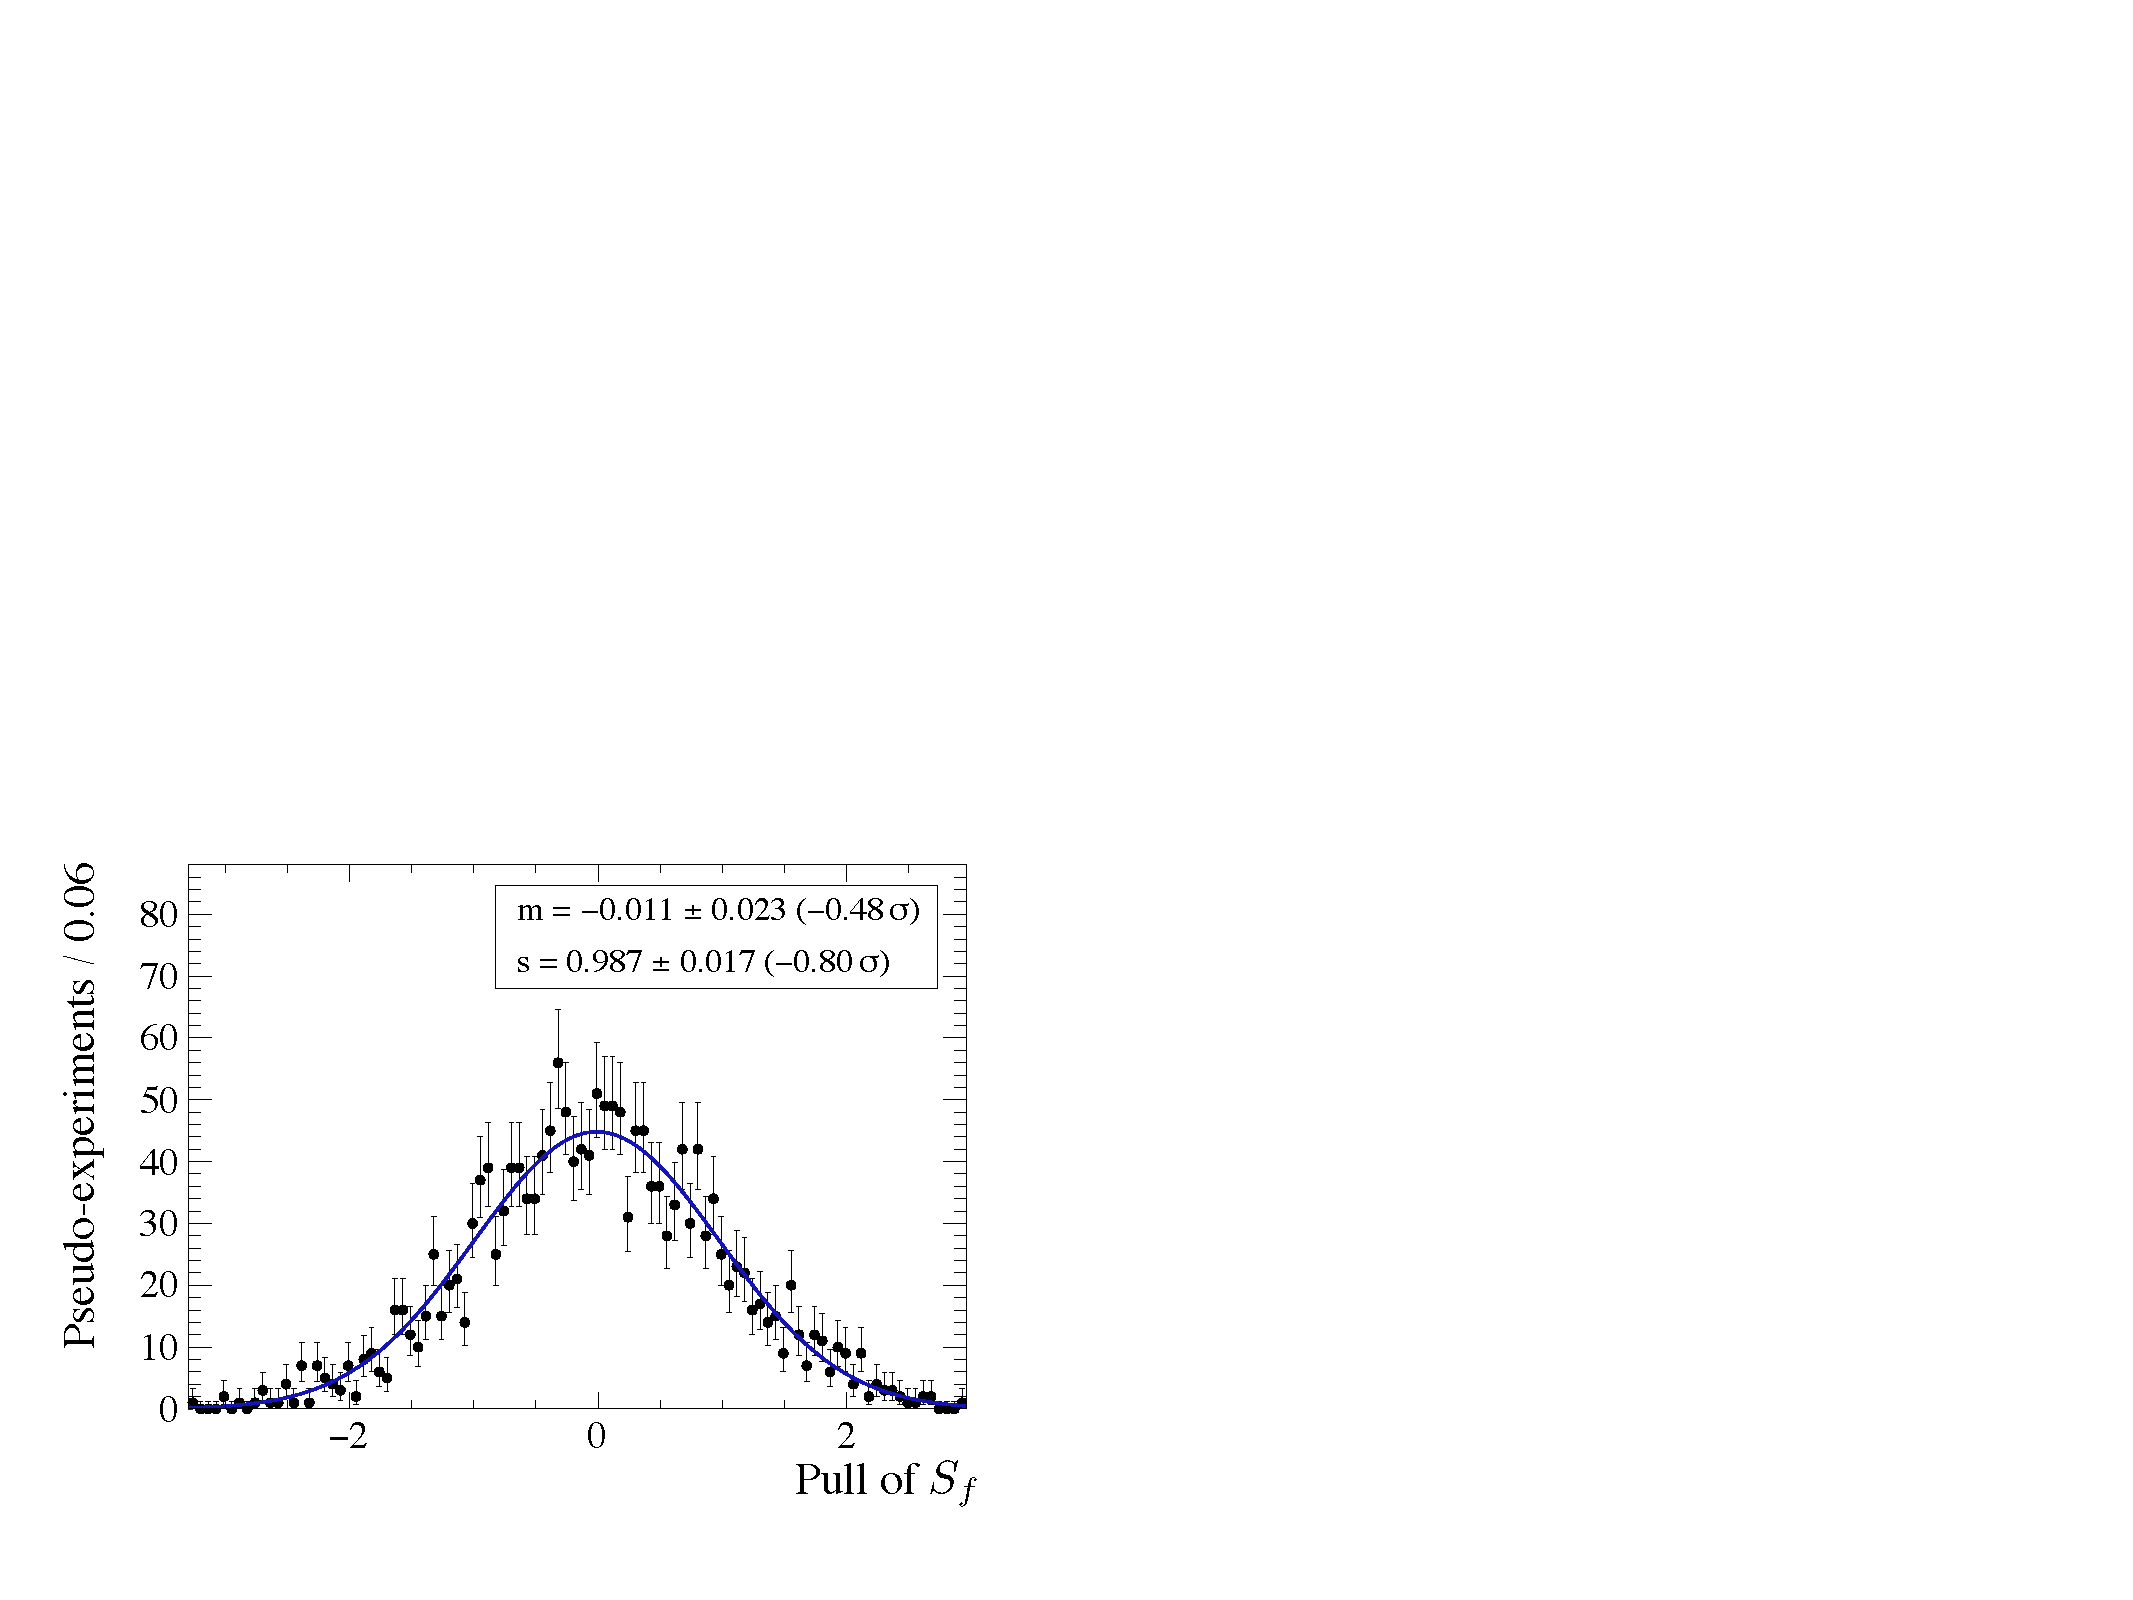
\includegraphics[width=0.48\textwidth]{10TimeFit/figs/Sf_pull_LinkValid_p1.pdf}
    	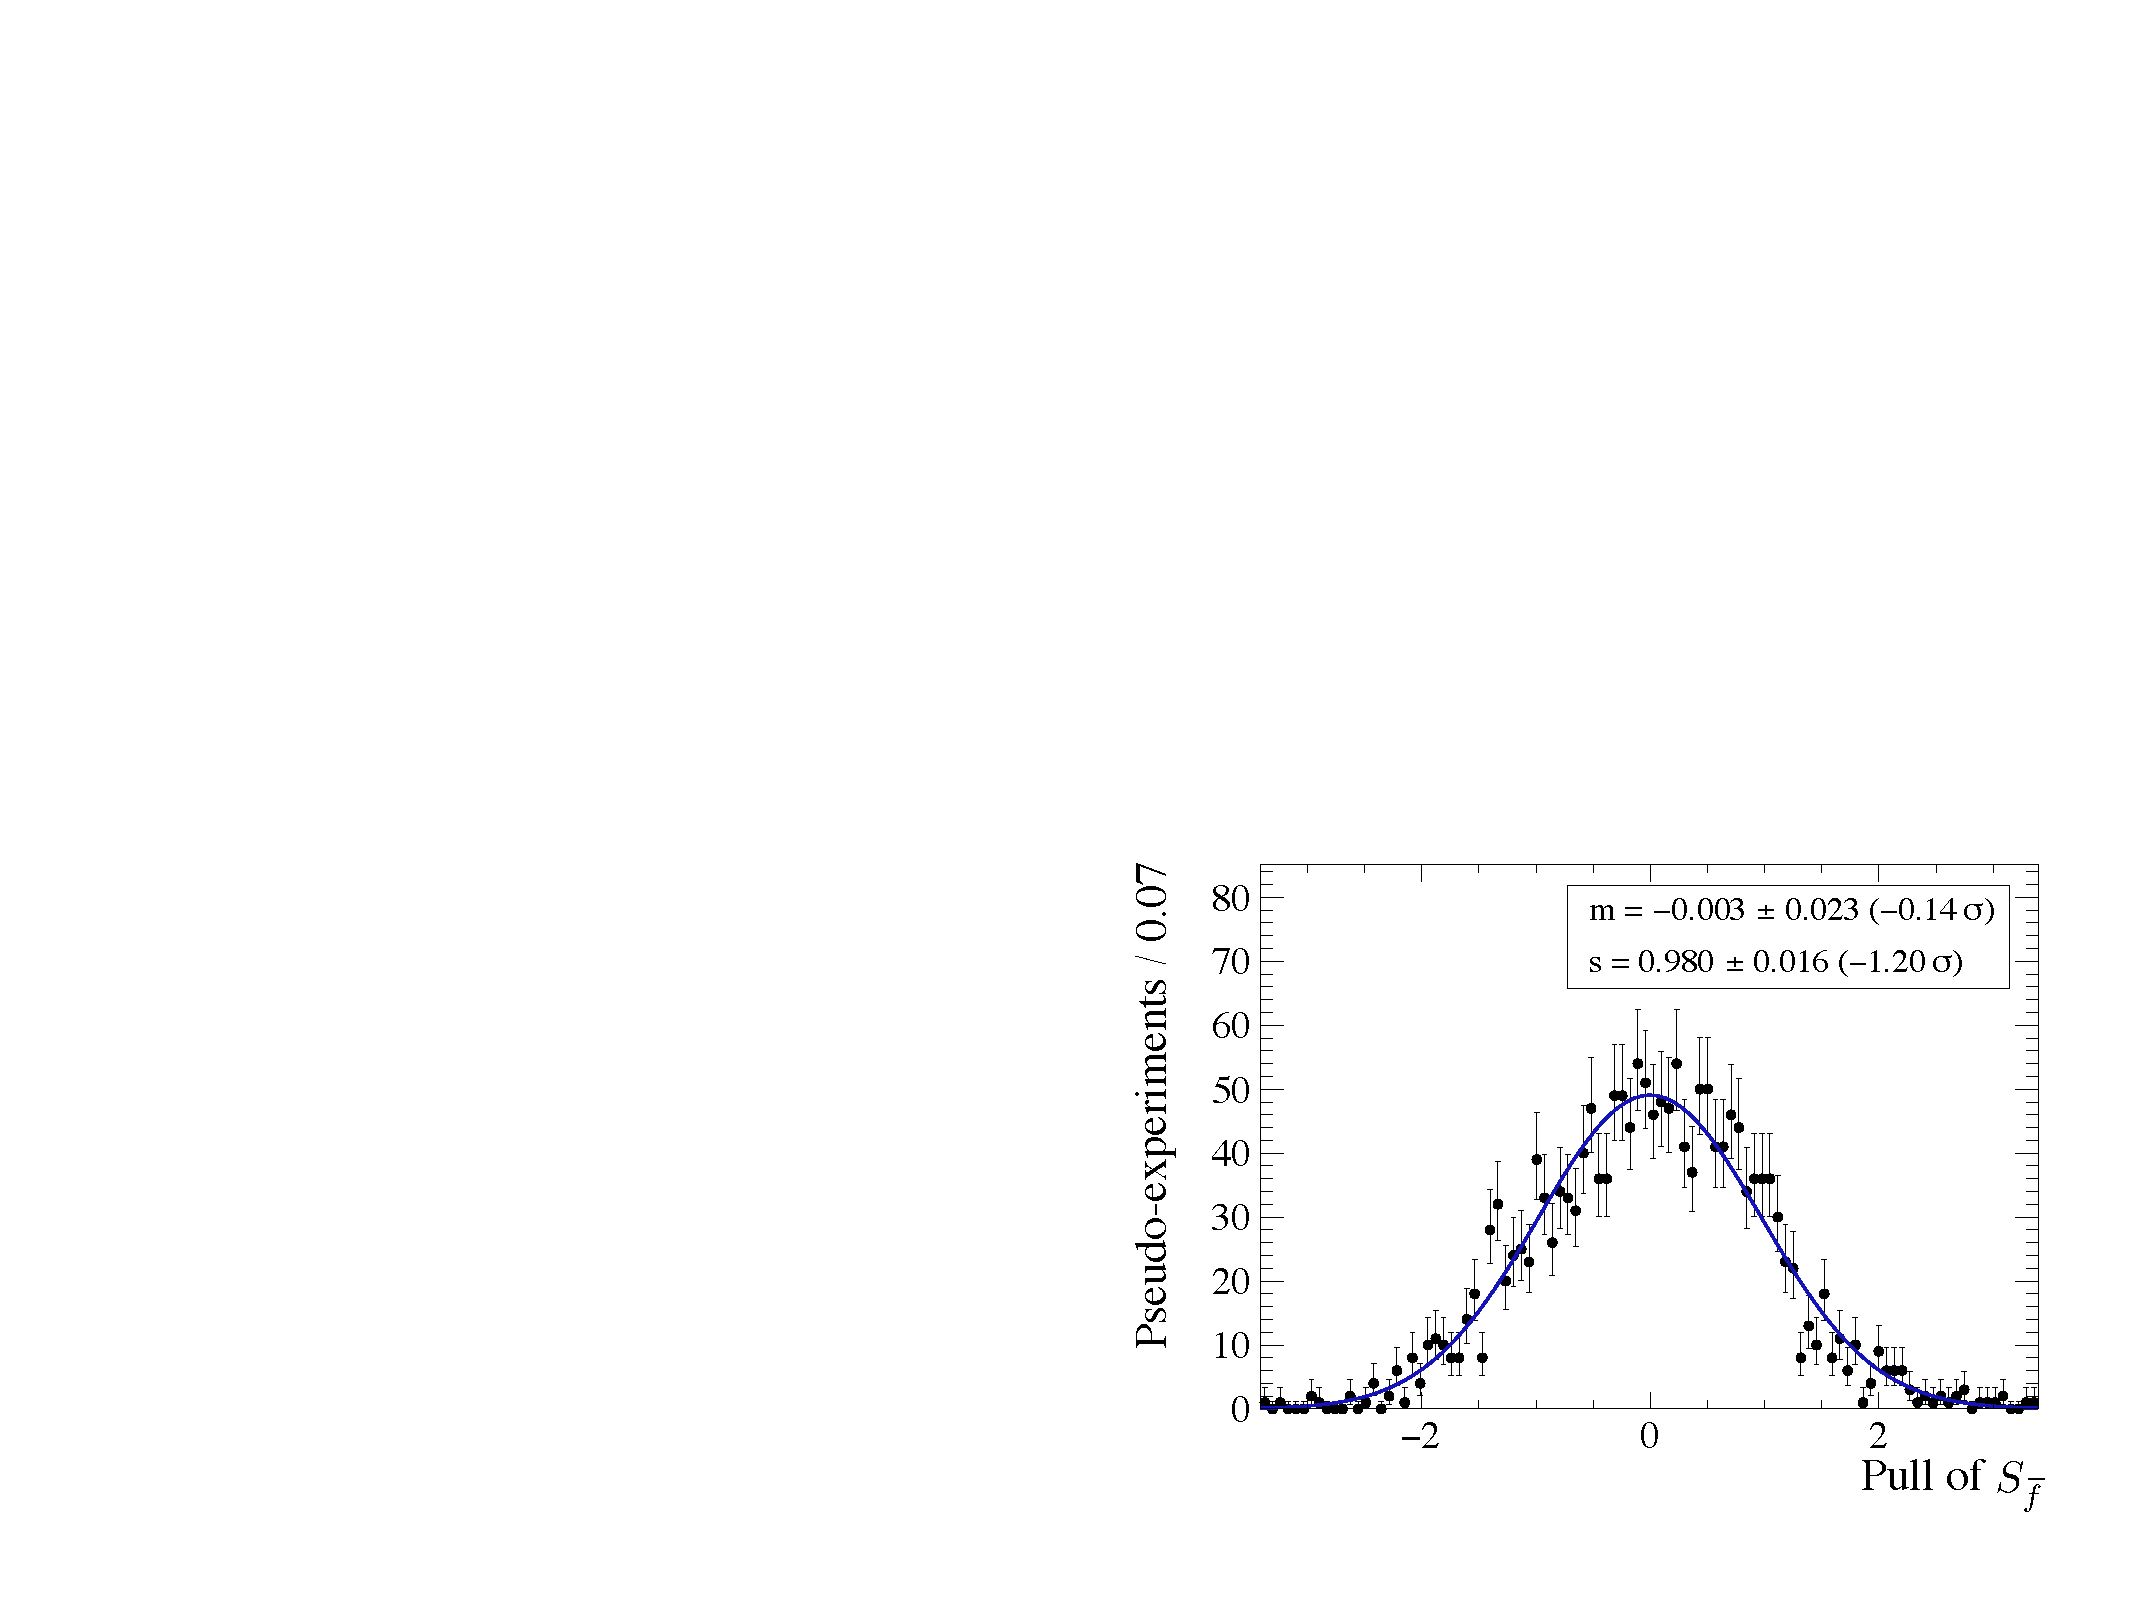
\includegraphics[width=0.48\textwidth]{10TimeFit/figs/Sfbar_pull_LinkValid_p1.pdf}
    \caption{Pull distributions of \Sf (left) and \Sfbar (right) when generating pseudoexperiments with artificially enlarged mistag asymmetry calibration parameters and a flip of the tag decision if $\omega'>0.5$ (top) and with the artificially enlarged parameter $p_1^{\text{\tiny OS}}$ and a flip of the tag decision if $\omega'>0.5$ (bottom).}
    \label{fig:linkFunctionValid}
\end{figure}

\newpage

	\item In a last study, the pseudoexeriments are generated with artificially increased tagging asymmetry parameters.
	But instead of flipping the tag decision, it is set to $d=0$ when the mistag probability exceeds \num{0.5}.
	In order to achieve a stable fit the distribution of estimated mistags $\eta$ for the OS and SS is reduced beforehand to
	\begin{equation}
	\eta<\frac{0.5-(p_0+\delta p_0)+(p_1+\delta p_1\left<\eta\right>}{p_1+\delta p_1}\,,
	\end{equation}
	where $\delta p_i$ are the uncertainties of the calibration parameters.
	This assures that the mistag probabilities do not exceed \num{0.5}.
	This strategy yields unbiased results for \Sf and \Sfbar.
\end{itemize}

From this studies, it can be concluded that the flip of the tag decision can bias the measurement of \CP parameters.
However, the size of the bias depends on the specific values of the calibration parameters and this needs to be studied for each specific set of values.
On the other hand, reducing the allowed range of estimated mistags prevents a bias on the measurement of \CP parameters, but depending on the cut that needs to be applied, this could reduce the statistical sensitivity of the analysis.
Therefore, the modified \emph{link function} as used in the nominal approach currently provides the best unbiased appraoch as will be shown in \cref{sec:valOnSim}.

\subsection{Cross checks on sub samples}
\label{sec:valOnSub Sample}

The stability of the fit is checked by also performing the fit in different sub samples of the full data set.
The data set is split in several ways, namely by data taking conditions, used tagging algorithms or kinematic properties of the \Bz meson and properties of the event.

When splitting according to data taking conditions, the \BdToDpi sample is divided by the year of data taking and magnetic polarity.
For each sub sample, the \emph{sWeights} are determined with a dedicated mass fit according to the procedure from \cref{ch:massfit}.
A comparison of the fitted values for \Sf and \Sfbar between the four sub samples is shown in \cref{fig:splitByDataTaking}.
The obtained results for \Sf and \Sfbar show good agreement and the average result from the fits in the sub samples is well compatible with the result of the nominal fit.
\begin{figure}[tbp]
    \centering
    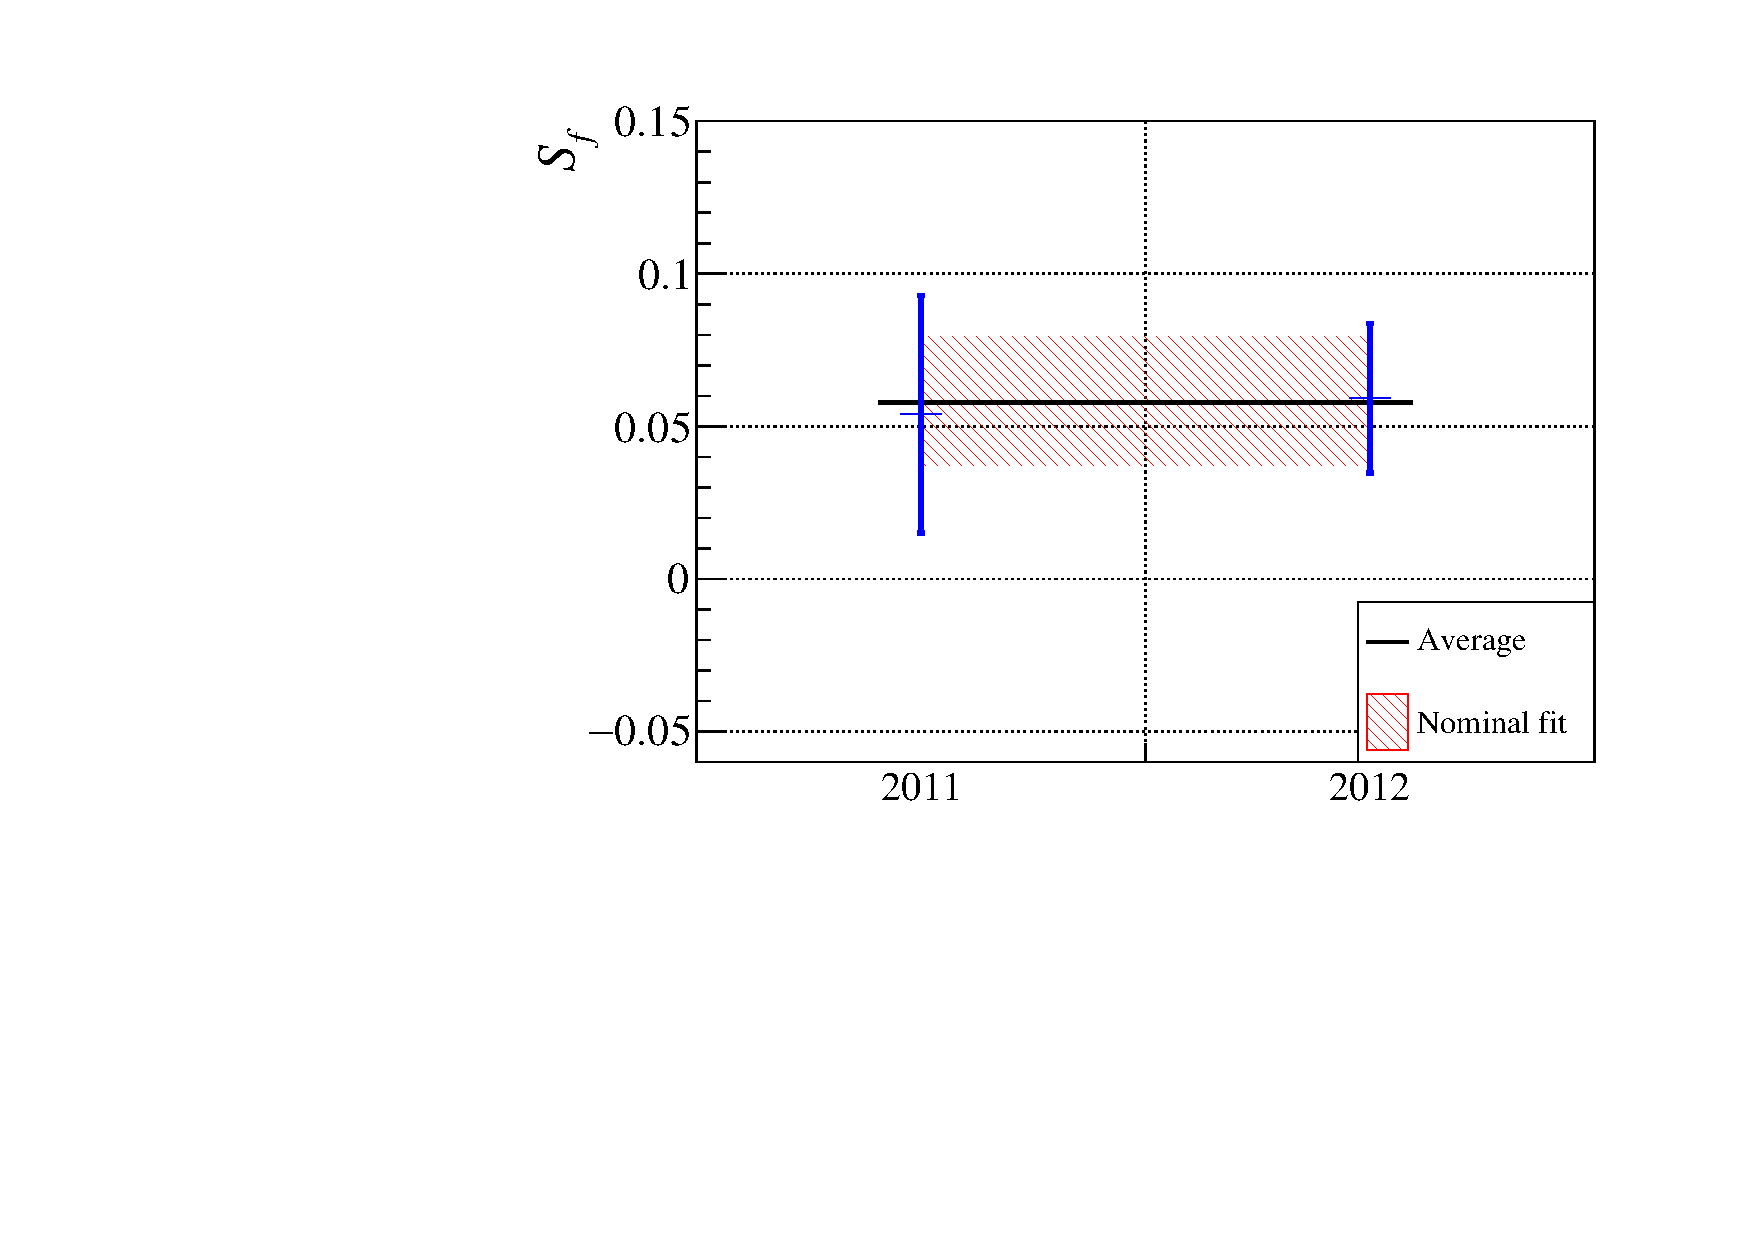
\includegraphics[width=0.48\textwidth]{10TimeFit/figs/Sf_splits_Year.pdf}
    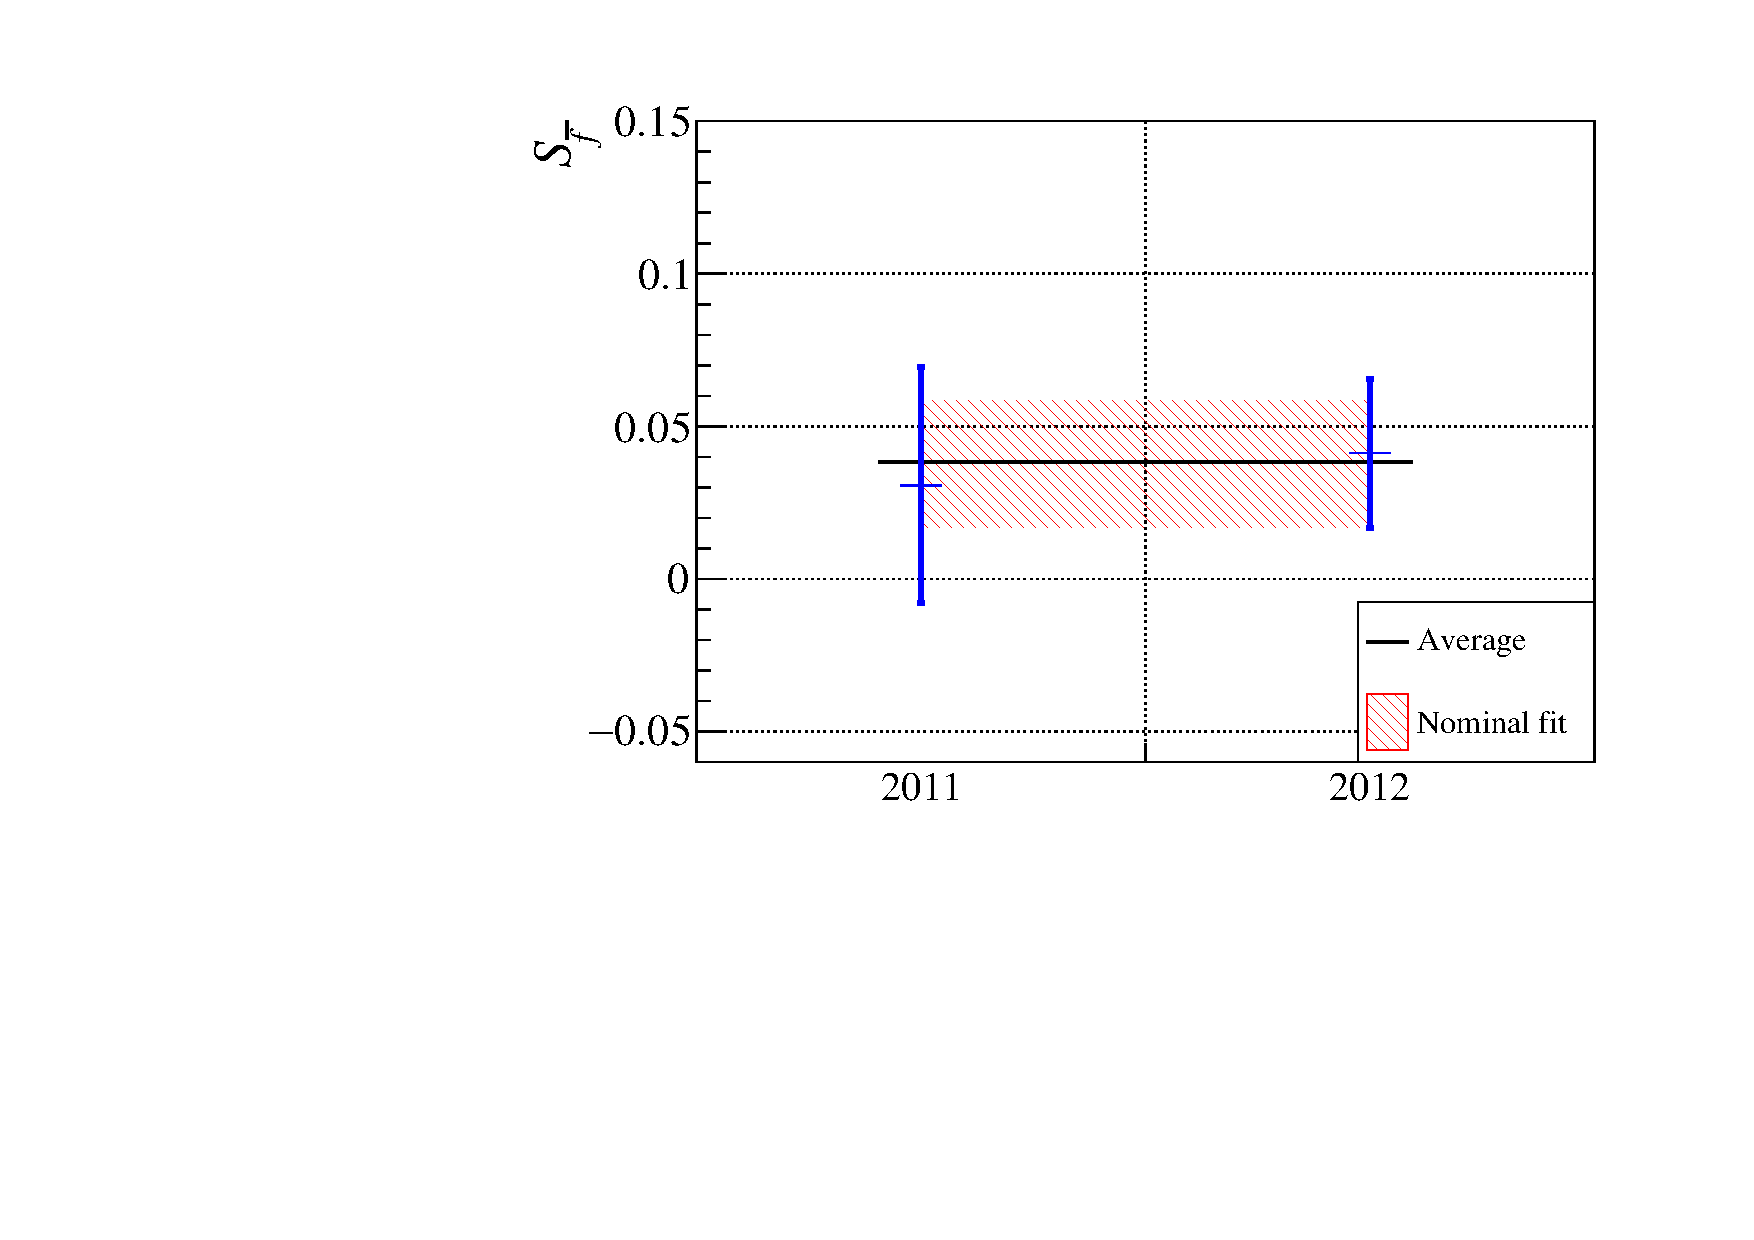
\includegraphics[width=0.48\textwidth]{10TimeFit/figs/Sfbar_splits_Year.pdf}\\
    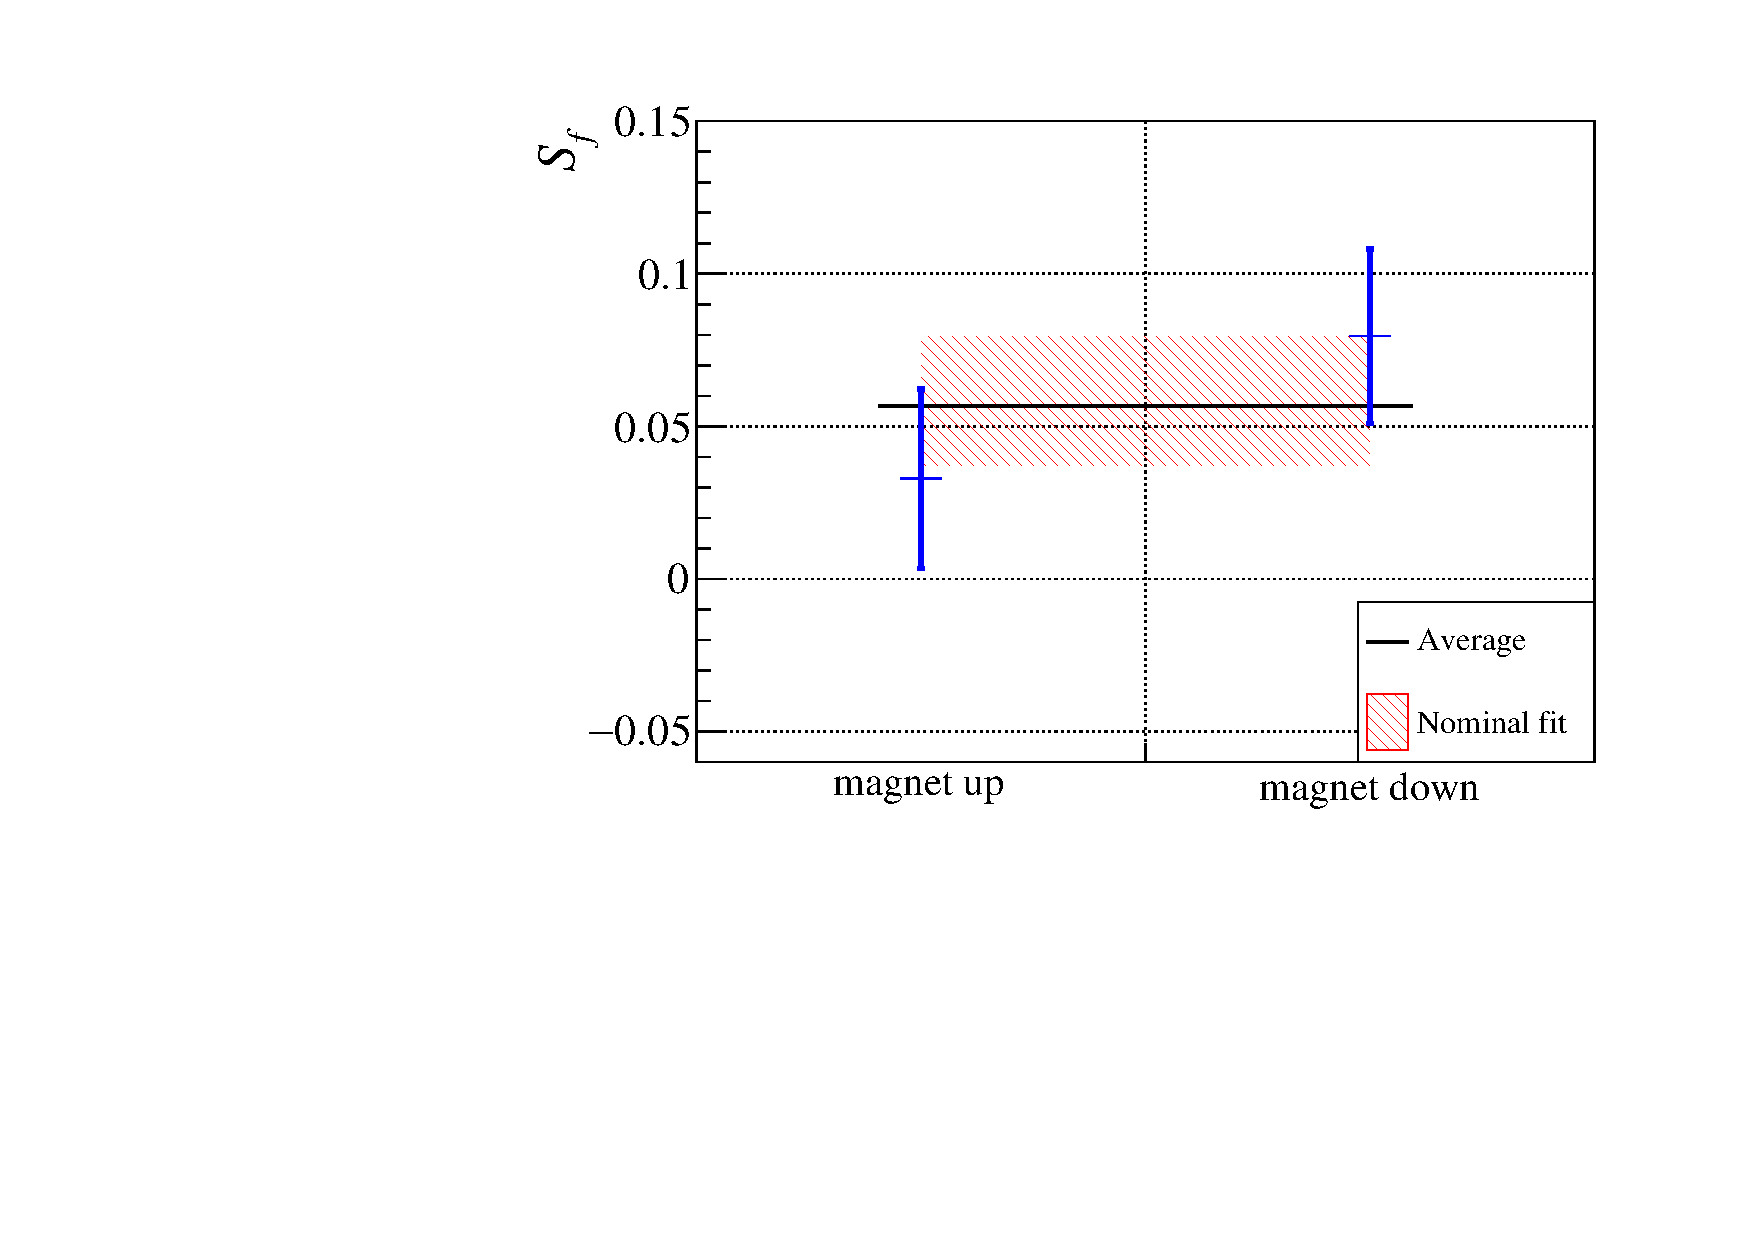
\includegraphics[width=0.48\textwidth]{10TimeFit/figs/Sf_splits_Polarity.pdf}
    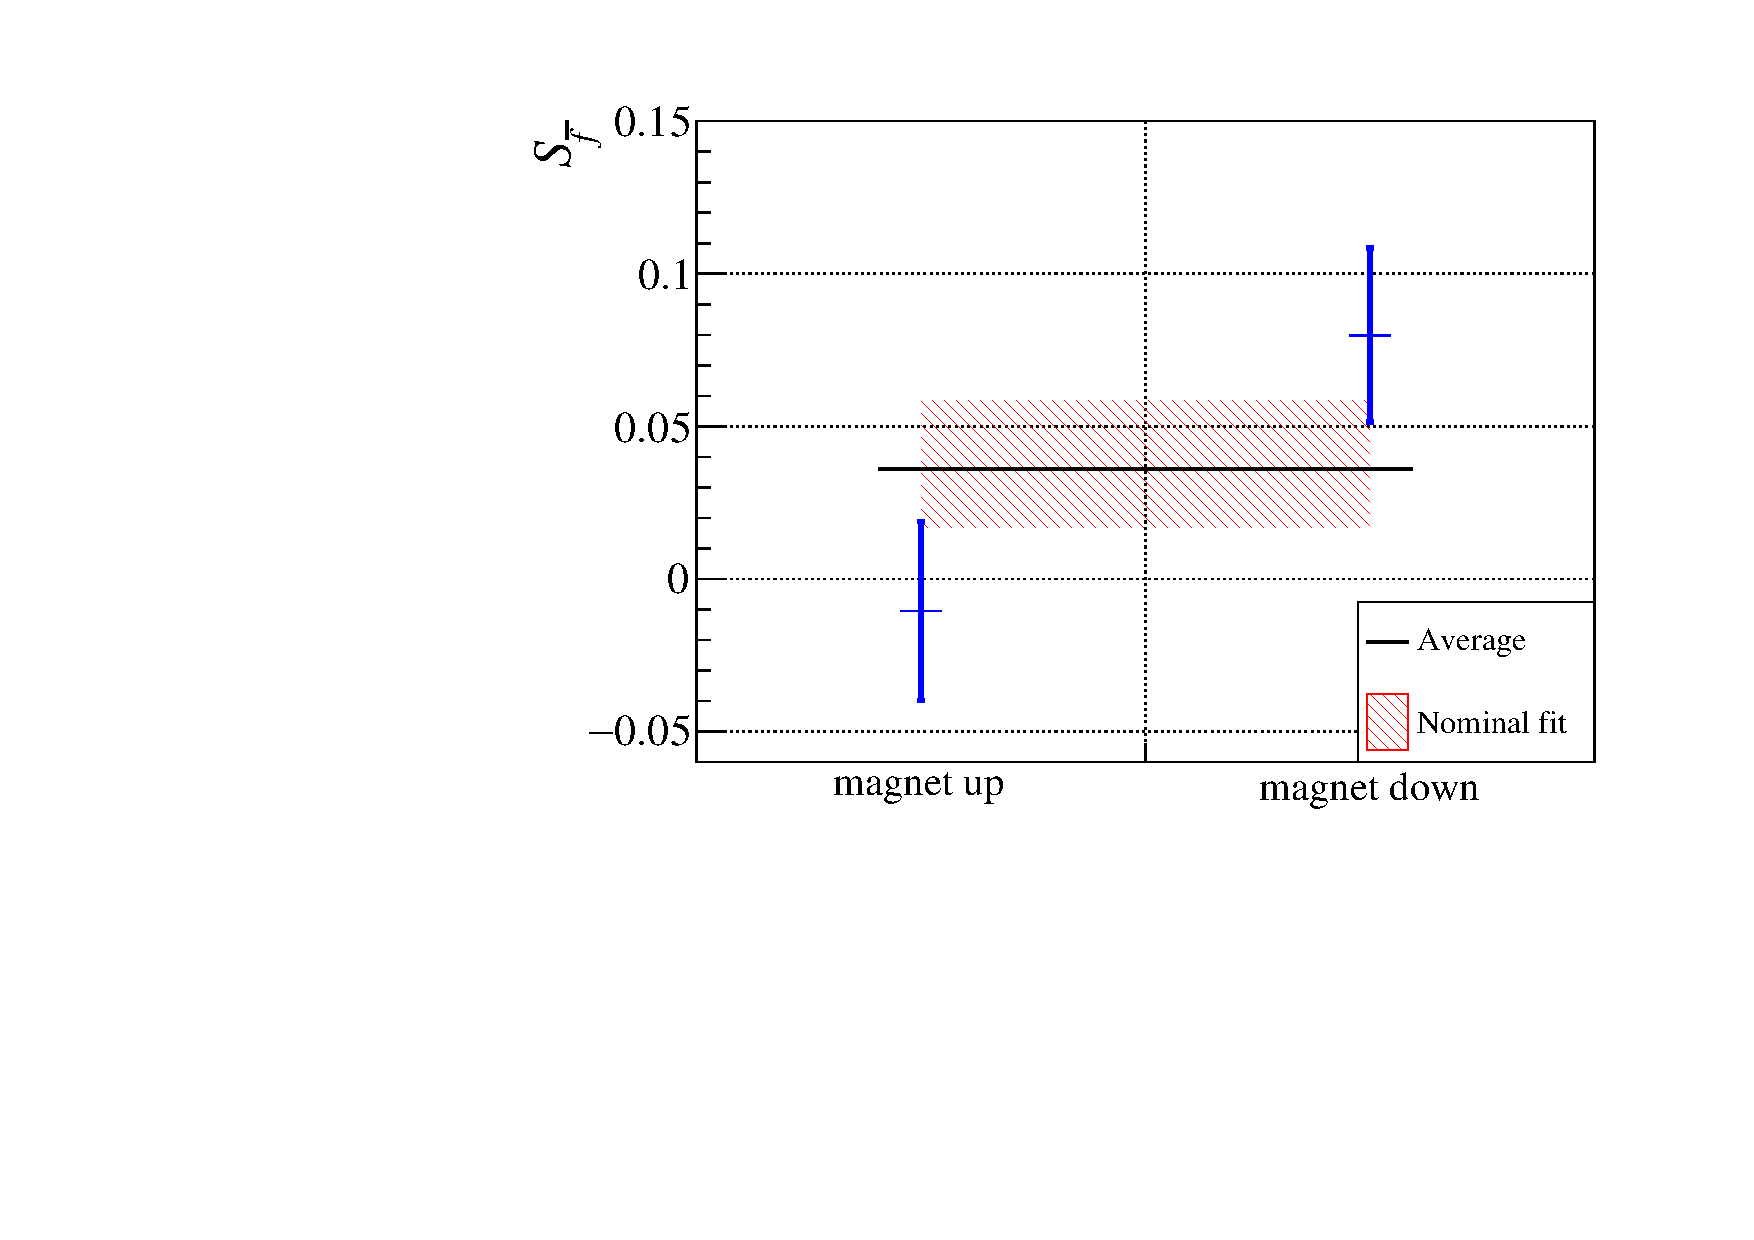
\includegraphics[width=0.48\textwidth]{10TimeFit/figs/Sfbar_splits_Polarity.pdf}
    \caption{Comparison between the fitted values of \Sf (left) and \Sfbar (right) in sub samples split by year of data taking (top) and magnet polarity (bottom).
    The blue points are the results of the fits in the sub samples, the red dashed area represents the result of the nominal fit and the black line is the average of the results obtained in the sub samples.}
    \label{fig:splitByDataTaking}
\end{figure}

When using two classes of tagging algorithms, the full sample is divided into three independent samples.
The first sub sample contains candidates tagged exclusively by the OS algorithms while the second sample consists of candidates which are only tagged by the SS algorithms.
The third class contains candidates which are tagged by both, OS taggers and SS taggers.
Again, the results for all sub samples show good agreement (see \cref{fig:splitByTagger}).
Furthermore, this agreement gives additional confidence that the strategy of floating the calibration parameters in the decay-time fit provides a stable result for the \CP parameters \Sf and \Sfbar.
\begin{figure}[tbp]
    \centering
    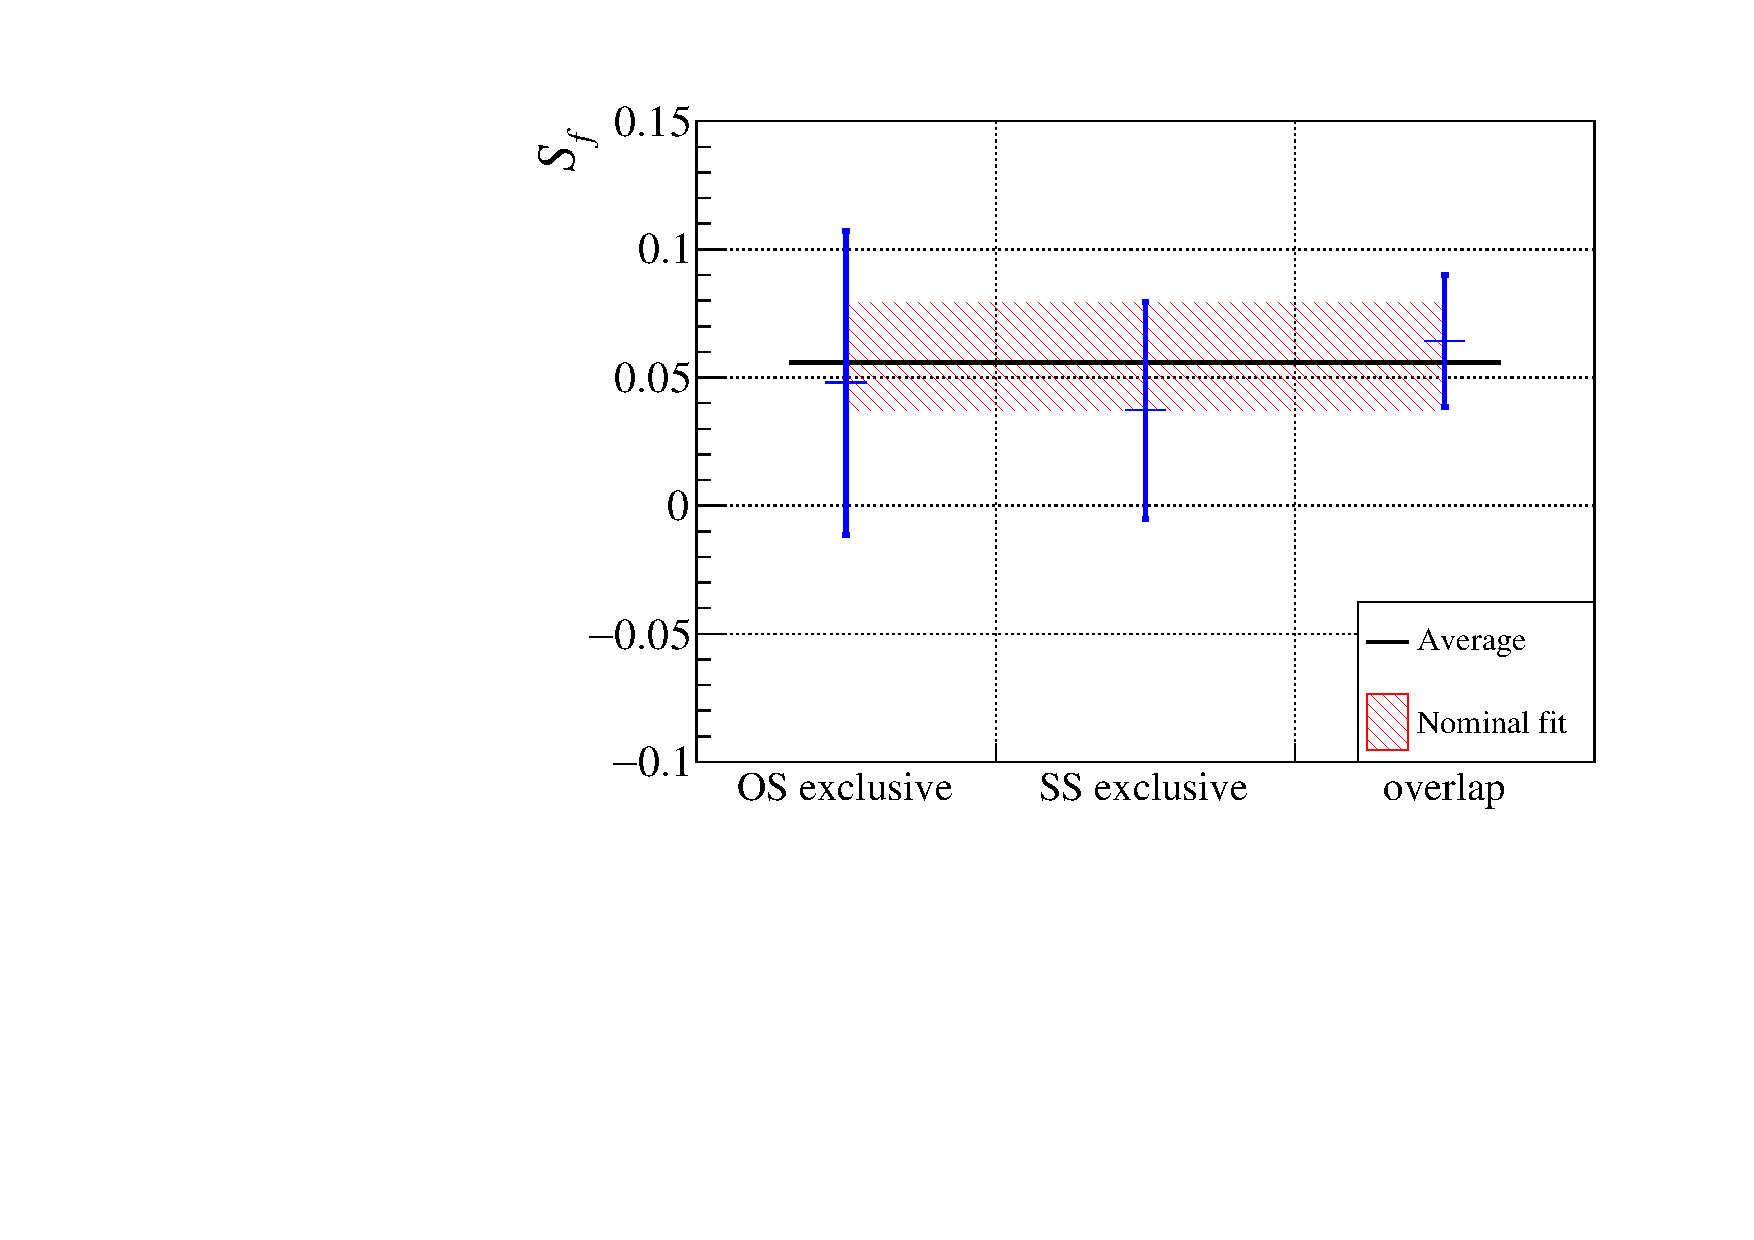
\includegraphics[width=0.48\textwidth]{10TimeFit/figs/Sf_splits_SSOSExclusive.pdf}
    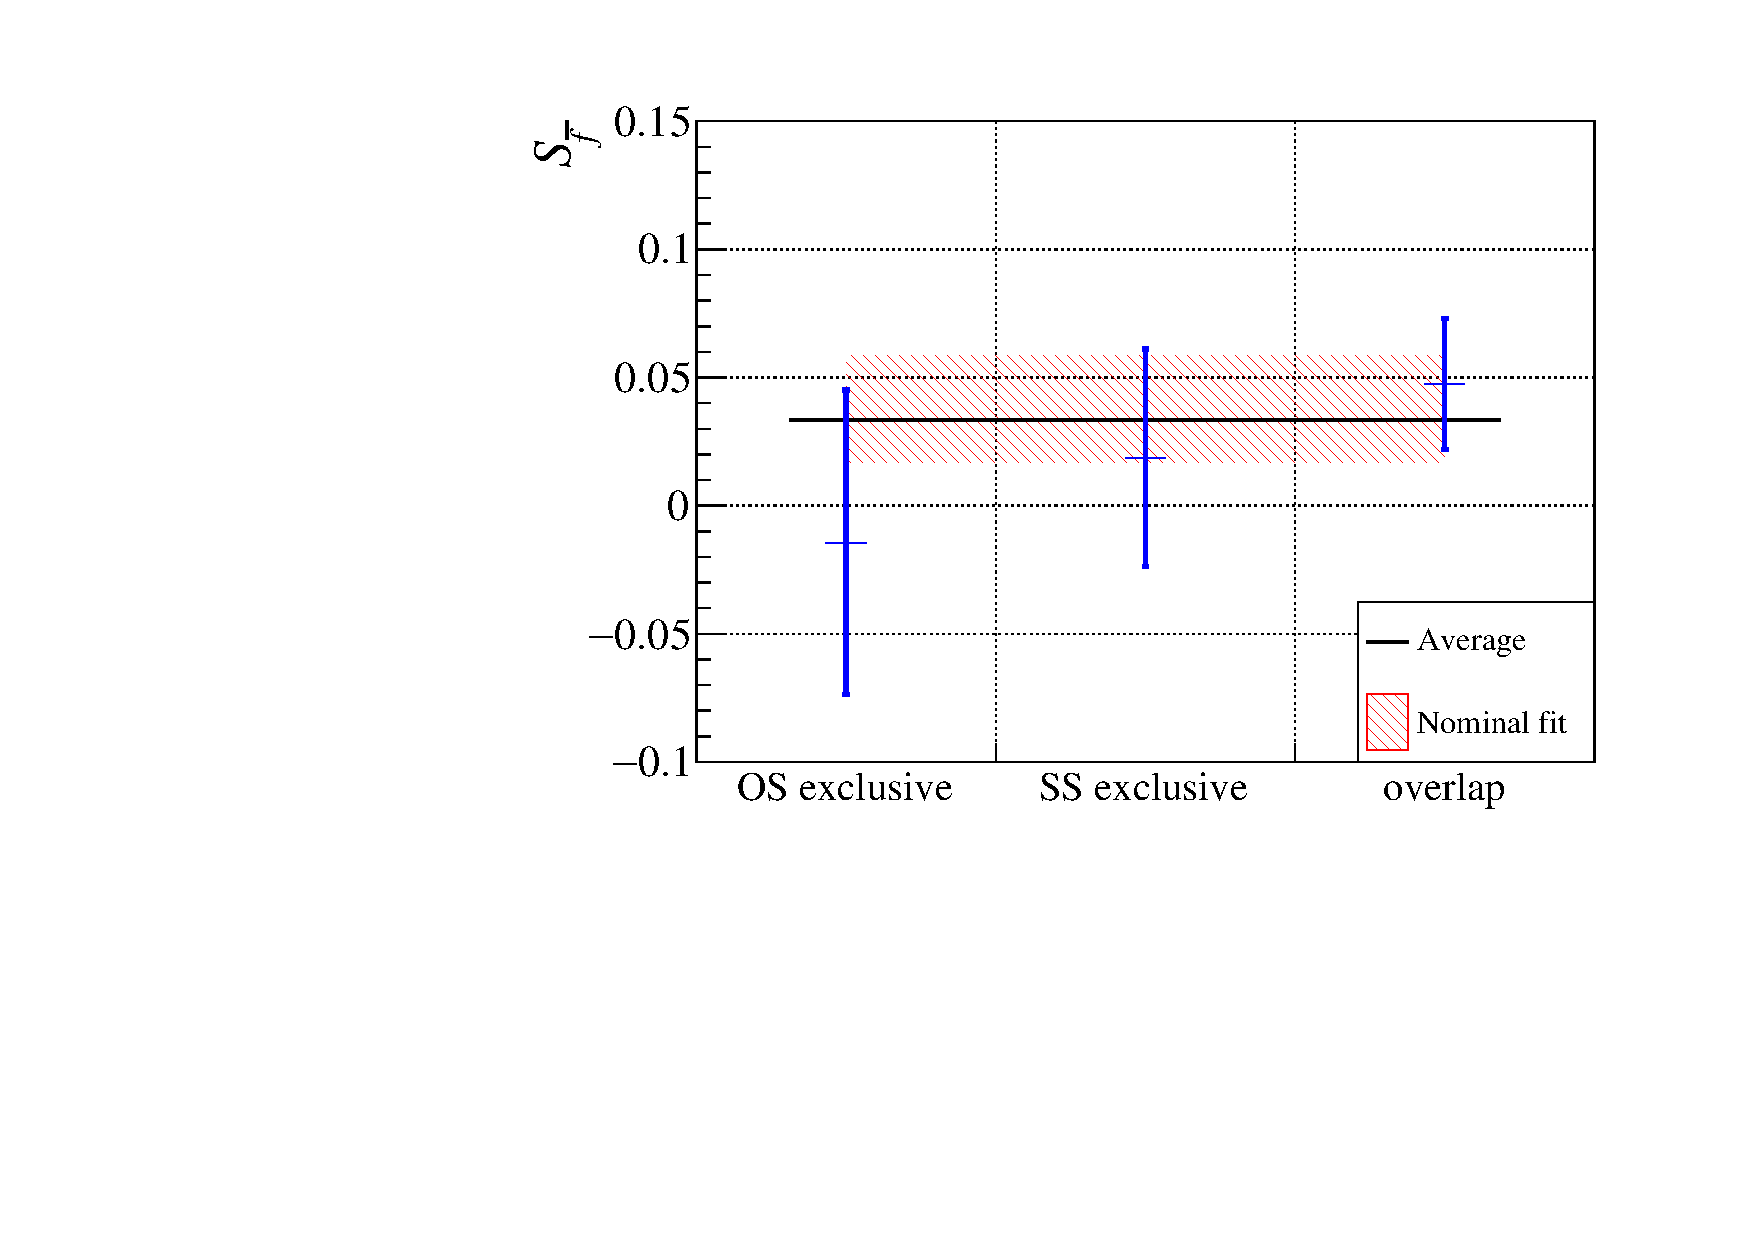
\includegraphics[width=0.48\textwidth]{10TimeFit/figs/Sfbar_splits_SSOSExclusive.pdf}
    \caption{Comparison between the fitted values of \Sf (left) and \Sfbar (right) when considering candidates exclusively tagged by the OS, SS or both classes of tagging algorithms.
    The blue points are the results of the fits in the sub samples, the red dashed area represents the result of the nominal fit and the black line is the average of the results obtained in the sub samples.}
    \label{fig:splitByTagger}
\end{figure}

Finally, the data set is split in four bins in the transverse momentum of the \Bz mesons, three bins in the number of reconstructed \ac{PV}s and tracks in the event and in four bins in the difference in pseudo-rapidity between the \Dpm meson and the bachelor particle.
The reason for these splits is that the flavour tagging calibrations partly depend on these observables, and therefore could cause a bias in the corresponding splits.
Moreover, the difference in pseudo-rapidity is also sensitive to possible misalignments in the detector, which could influence the measurement of \Sf and \Sfbar.
However, all results show compatible results and no trends are observed.

\subsection{Decay-time fits to simulated events}
\label{sec:valOnSim}

To validate the fit using simulated events, these are bootstrapped, \ie the simulated data sample is resampled $n$ times, whereby it is allowed that single events can be taken more than once, \eg a bootstrapped sample can contain the same event multiple times.
This is statistically valid because individual events are not correlated with each other.
Each generated sample then contains as many candidates as signal candidates in the full \BdToDpi data sample used in \cref{sec:ExtractCPobs} in order to obtain the same statistical uncertainties.

After generation, the samples are fitted with the same strategy as the nominal fit to extract the \CP observables.
The constrained parameters $\tau$ and \dm are treated as follows:
for each fit, a value is generated randomly from the respective Gaussian function with which $\tau$ and \dm are constrained.
This new value is then used in the fit as the mean value of the constraints.
This allows the correct fluctuation for both parameters and prevents an underestimation of the fitted uncertainties.
For the nominal constraint, the generation values of the simulated sample are used as the mean value, while for the width, the same value as on data is used.
This means that the lifetime is constrained to $\tau=\SI{1.519\pm0.004}{\pico\second}$ and the oscillation frequency to $\dm=\SI{0.5100\pm0.0023}{\per\pico\second}$.

For all settings described below, the distributions of residuals are studied for \Sf and \Sfbar, whereby the residual is defined as the fitted value minus the value used in the generation  of the simulated sample.
This residual distributions are fitted with a Gaussian function in order to determine the mean and width.
A mean value deviating from zero hints to a biased result, while the width of the distribution allows to determine the expected uncertainty of the parameter.
Performing such a study with \num{1000} bootstrapped samples with the nominal strategy yields a mean of \num{0.0064\pm0.0007} for \Sf and \num{-0.0024\pm0.0007} for \Sfbar.
This corresponds to a deviation of roughly one third of the statistical uncertainty for \Sf and about \SI{10}{\percent} of the statistical uncertainty for \Sfbar  as shown in \cref{fig:BootstrapStudy}.
\begin{figure}[tbp]
    \centering
    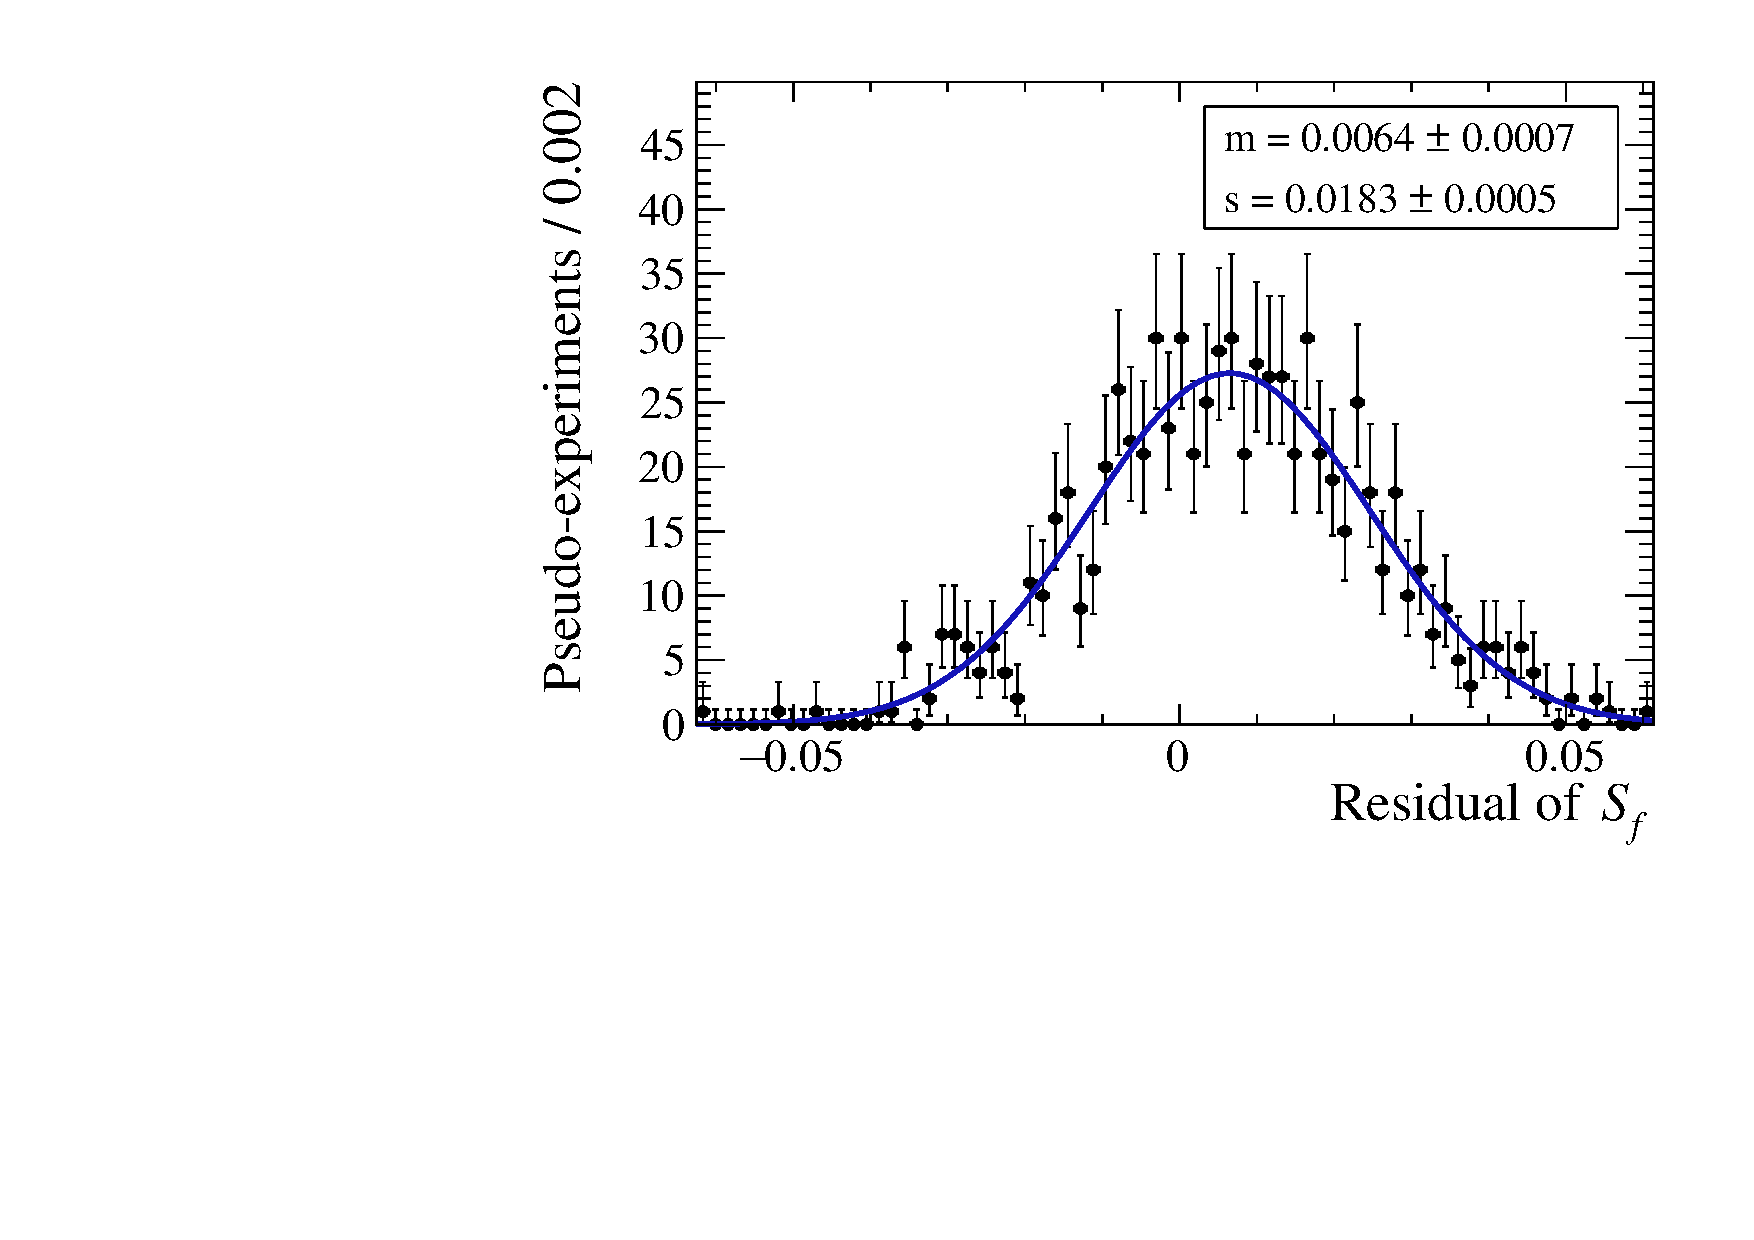
\includegraphics[width=0.48\textwidth]{10TimeFit/figs/S_f_res.pdf}
    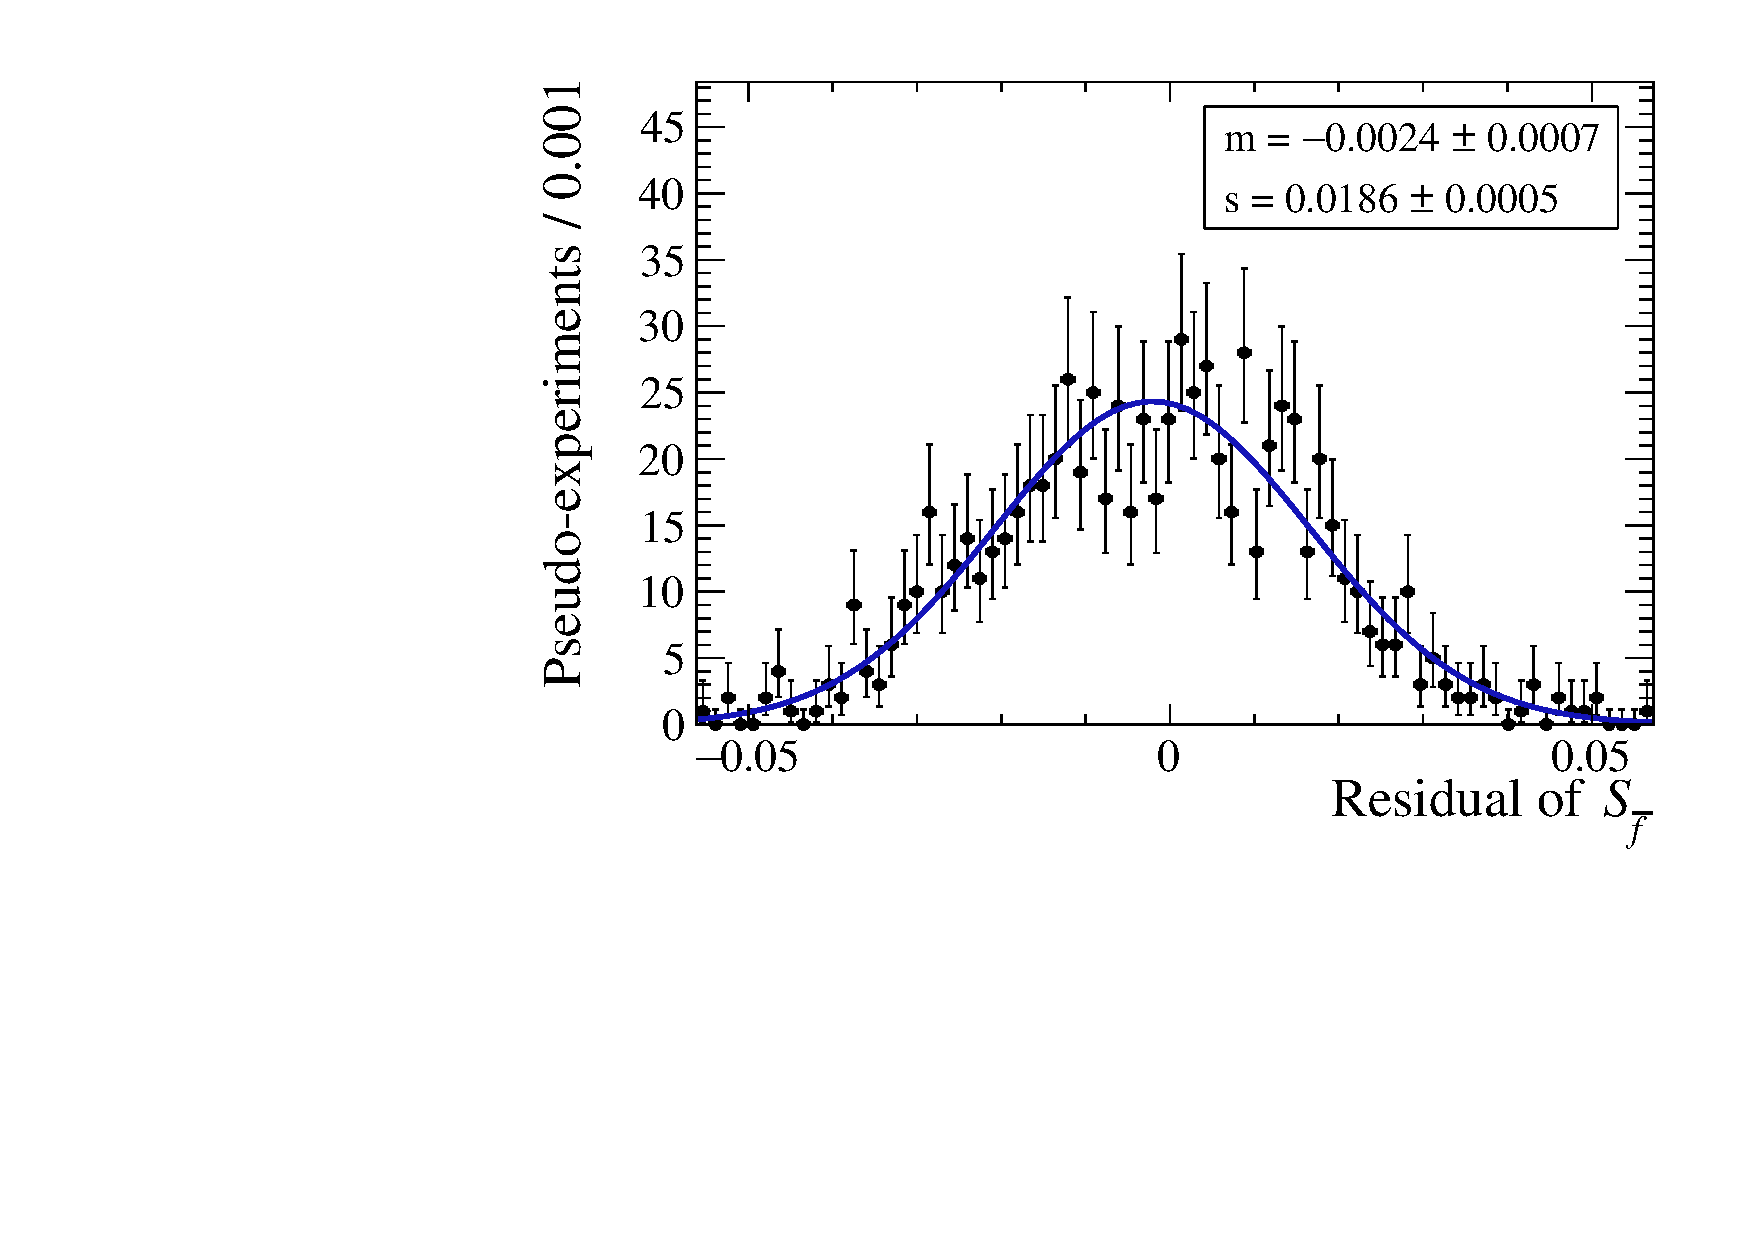
\includegraphics[width=0.48\textwidth]{10TimeFit/figs/S_fbar_res.pdf}
    \caption{Distribution of residuals for \Sf (left) and \Sfbar (right) using the nominal fit strategy with floating calibration.}
    \label{fig:BootstrapStudy}
\end{figure}
Furthermore, the following configurations are also investigated with \num{1000} bootstrapped samples each:

\newpage

\begin{itemize}
	\item Using the true generated flavour of the \B candidate instead of the tag decision and mistag estimate provided by the real tagging algorithms leads to an unbiased distribution of residuals for \Sf and \Sfbar.
	\item A \emph{cheated} tagger is implemented for simulated data.
	Instead of using the perfect tagging as in the first appraoch, the truth information for each candidate is resampled depending on the mistag probability.
	This way, the mistag is used as a conditional observable as is done in the nominal fit, but still the truth information from the simulation is exploited.
	This appraoch also gives unbiased results for \Sf and \Sfbar.
	\item The retraining of the SS tagging algorithms is performed on simulated samples in the same way as described in \cref{sec:SScalibration}.
	Afterwards, the calibration for the OS and SS algorithms is obtained from \BdToDpi using the true generated flavour as done for the portability checks in \cref{sec:SScalibration} and \cref{sec:OScalibration}.
	Performing the fits to the bootstrapped simulation samples of \BdToDpi, no bias on \Sf and \Sfbar is observed.
	\item The retraining and calibration of the tagging algorithms is performed on simulated samples in the same way as described in \cref{sec:SScalibration} and \cref{sec:OScalibration}.
	This calibration is applied in the fits to the bootstrapped simulation samples of \BdToDpi, what leads to a bias on \Sf and \Sfbar of the size of the statistical uncertainty of both parameters.
	\item Instead of fixing the calibration parameters obtained on simulated samples, they are constrained by means of Gaussian functions in the decay-time fits to the  bootstrapped simulation samples of \BdToDpi .
	These constraints are implented by multidimensional Gaussian functions taking into account the correlations on the simulated control samples.
	This approach reduces the bias on \Sf and \Sfbar to a value of the order of half the statistical uncertainty of both parameters.
\end{itemize}
This confirms that leaving the flavour tagging calibration parameters free in the \CP-fit is the best choice.
However, since the source of this potential, but anyway small bias cannot be narrowed down further than coming from the flavour tagging calibration, it is included as systematic uncertainty.
To confirm the size of the bias, a second study was performed by a collaborator yielding as mean values of the distribution of residuals \num{0.0071\pm0.0006} and \num{-0.0013\pm0.0006} for \Sf and \Sfbar, respectively.
Finally, the average value from both studies, \ie \num{0.0068\pm0.0005} for \Sf and \num{-0.0018\pm0.0005} for \Sfbar is assumed as systematic uncertainty (see \cref{ch:systeamticUncerts}).
